\chapter{More about Types}
\label{ch:more-types}

So far we have learned about a few basic types (for example \isa{bool} and
\isa{nat}), type abbreviations (\isacommand{types}) and recursive datatypes
(\isacommand{datatype}). This chapter will introduce more
advanced material:
\begin{itemize}
\item Pairs ({\S}\ref{sec:products}) and records ({\S}\ref{sec:records}),
and how to reason about them.
\item Type classes: how to specify and reason about axiomatic collections of
  types ({\S}\ref{sec:axclass}). This section leads on to a discussion of
  Isabelle's numeric types ({\S}\ref{sec:numbers}).  
\item Introducing your own types: how to define types that
  cannot be constructed with any of the basic methods
  ({\S}\ref{sec:adv-typedef}).
\end{itemize}

The material in this section goes beyond the needs of most novices.
Serious users should at least skim the sections as far as type classes.
That material is fairly advanced; read the beginning to understand what it
is about, but consult the rest only when necessary.

\index{pairs and tuples|(}
%
\begin{isabellebody}%
\def\isabellecontext{Pairs}%
\isamarkupfalse%
%
\isamarkupsection{Pairs and Tuples%
}
\isamarkuptrue%
%
\begin{isamarkuptext}%
\label{sec:products}
Ordered pairs were already introduced in \S\ref{sec:pairs}, but only with a minimal
repertoire of operations: pairing and the two projections \isa{fst} and
\isa{snd}. In any non-trivial application of pairs you will find that this
quickly leads to unreadable nests of projections. This
section introduces syntactic sugar to overcome this
problem: pattern matching with tuples.%
\end{isamarkuptext}%
\isamarkuptrue%
%
\isamarkupsubsection{Pattern Matching with Tuples%
}
\isamarkuptrue%
%
\begin{isamarkuptext}%
Tuples may be used as patterns in $\lambda$-abstractions,
for example \isa{{\isasymlambda}{\isacharparenleft}x{\isacharcomma}y{\isacharcomma}z{\isacharparenright}{\isachardot}x{\isacharplus}y{\isacharplus}z} and \isa{{\isasymlambda}{\isacharparenleft}{\isacharparenleft}x{\isacharcomma}y{\isacharparenright}{\isacharcomma}z{\isacharparenright}{\isachardot}x{\isacharplus}y{\isacharplus}z}. In fact,
tuple patterns can be used in most variable binding constructs,
and they can be nested. Here are
some typical examples:
\begin{quote}
\isa{let\ {\isacharparenleft}x{\isacharcomma}\ y{\isacharparenright}\ {\isacharequal}\ f\ z\ in\ {\isacharparenleft}y{\isacharcomma}\ x{\isacharparenright}}\\
\isa{case\ xs\ of\ {\isacharbrackleft}{\isacharbrackright}\ {\isasymRightarrow}\ {\isadigit{0}}\ {\isacharbar}\ {\isacharparenleft}x{\isacharcomma}\ y{\isacharparenright}\ {\isacharhash}\ zs\ {\isasymRightarrow}\ x\ {\isacharplus}\ y}\\
\isa{{\isasymforall}{\isacharparenleft}x{\isacharcomma}y{\isacharparenright}{\isasymin}A{\isachardot}\ x{\isacharequal}y}\\
\isa{{\isacharbraceleft}{\isacharparenleft}x{\isacharcomma}y{\isacharcomma}z{\isacharparenright}{\isachardot}\ x{\isacharequal}z{\isacharbraceright}}\\
\isa{{\isasymUnion}\isactrlbsub {\isacharparenleft}x{\isacharcomma}\ y{\isacharparenright}{\isasymin}A\isactrlesub \ {\isacharbraceleft}x\ {\isacharplus}\ y{\isacharbraceright}}
\end{quote}
The intuitive meanings of these expressions should be obvious.
Unfortunately, we need to know in more detail what the notation really stands
for once we have to reason about it.  Abstraction
over pairs and tuples is merely a convenient shorthand for a more complex
internal representation.  Thus the internal and external form of a term may
differ, which can affect proofs. If you want to avoid this complication,
stick to \isa{fst} and \isa{snd} and write \isa{{\isasymlambda}p{\isachardot}\ fst\ p\ {\isacharplus}\ snd\ p}
instead of \isa{{\isasymlambda}{\isacharparenleft}x{\isacharcomma}y{\isacharparenright}{\isachardot}\ x{\isacharplus}y}.  These terms are distinct even though they
denote the same function.

Internally, \isa{{\isasymlambda}{\isacharparenleft}x{\isacharcomma}\ y{\isacharparenright}{\isachardot}\ t} becomes \isa{split\ {\isacharparenleft}{\isasymlambda}x\ y{\isachardot}\ t{\isacharparenright}}, where
\cdx{split} is the uncurrying function of type \isa{{\isacharparenleft}{\isacharprime}a\ {\isasymRightarrow}\ {\isacharprime}b\ {\isasymRightarrow}\ {\isacharprime}c{\isacharparenright}\ {\isasymRightarrow}\ {\isacharprime}a\ {\isasymtimes}\ {\isacharprime}b\ {\isasymRightarrow}\ {\isacharprime}c} defined as
\begin{center}
\isa{split\ {\isasymequiv}\ {\isasymlambda}c\ p{\isachardot}\ c\ {\isacharparenleft}fst\ p{\isacharparenright}\ {\isacharparenleft}snd\ p{\isacharparenright}}
\hfill(\isa{split{\isacharunderscore}def})
\end{center}
Pattern matching in
other variable binding constructs is translated similarly. Thus we need to
understand how to reason about such constructs.%
\end{isamarkuptext}%
\isamarkuptrue%
%
\isamarkupsubsection{Theorem Proving%
}
\isamarkuptrue%
%
\begin{isamarkuptext}%
The most obvious approach is the brute force expansion of \isa{split}:%
\end{isamarkuptext}%
\isamarkuptrue%
\isacommand{lemma}\ {\isachardoublequote}{\isacharparenleft}{\isasymlambda}{\isacharparenleft}x{\isacharcomma}y{\isacharparenright}{\isachardot}x{\isacharparenright}\ p\ {\isacharequal}\ fst\ p{\isachardoublequote}\isanewline
\isamarkupfalse%
\isamarkupfalse%
%
\begin{isamarkuptext}%
This works well if rewriting with \isa{split{\isacharunderscore}def} finishes the
proof, as it does above.  But if it does not, you end up with exactly what
we are trying to avoid: nests of \isa{fst} and \isa{snd}. Thus this
approach is neither elegant nor very practical in large examples, although it
can be effective in small ones.

If we consider why this lemma presents a problem, 
we quickly realize that we need to replace the variable~\isa{p} by some pair \isa{{\isacharparenleft}a{\isacharcomma}\ b{\isacharparenright}}.  Then both sides of the
equation would simplify to \isa{a} by the simplification rules
\isa{split\ c\ {\isacharparenleft}a{\isacharcomma}\ b{\isacharparenright}\ {\isacharequal}\ c\ a\ b} and \isa{fst\ {\isacharparenleft}a{\isacharcomma}\ b{\isacharparenright}\ {\isacharequal}\ a}.  
To reason about tuple patterns requires some way of
converting a variable of product type into a pair.

In case of a subterm of the form \isa{split\ f\ p} this is easy: the split
rule \isa{split{\isacharunderscore}split} replaces \isa{p} by a pair:%
\index{*split (method)}%
\end{isamarkuptext}%
\isamarkuptrue%
\isacommand{lemma}\ {\isachardoublequote}{\isacharparenleft}{\isasymlambda}{\isacharparenleft}x{\isacharcomma}y{\isacharparenright}{\isachardot}y{\isacharparenright}\ p\ {\isacharequal}\ snd\ p{\isachardoublequote}\isanewline
\isamarkupfalse%
\isamarkupfalse%
\isamarkuptrue%
\isanewline
\isamarkupfalse%
\isamarkupfalse%
\isamarkupfalse%
%
\begin{isamarkuptext}%
Let us look at a second example:%
\end{isamarkuptext}%
\isamarkuptrue%
\isacommand{lemma}\ {\isachardoublequote}let\ {\isacharparenleft}x{\isacharcomma}y{\isacharparenright}\ {\isacharequal}\ p\ in\ fst\ p\ {\isacharequal}\ x{\isachardoublequote}\isanewline
\isamarkupfalse%
\isamarkupfalse%
\isamarkuptrue%
\isamarkupfalse%
\isacommand{lemma}\ {\isachardoublequote}p\ {\isasymin}\ {\isacharbraceleft}{\isacharparenleft}x{\isacharcomma}y{\isacharparenright}{\isachardot}\ x{\isacharequal}y{\isacharbraceright}\ {\isasymlongrightarrow}\ fst\ p\ {\isacharequal}\ snd\ p{\isachardoublequote}\isanewline
\isamarkupfalse%
\isamarkupfalse%
\isamarkuptrue%
\isamarkupfalse%
\isacommand{lemma}\ {\isachardoublequote}p\ {\isasymin}\ {\isacharbraceleft}{\isacharparenleft}x{\isacharcomma}y{\isacharparenright}{\isachardot}\ x{\isacharequal}y{\isacharbraceright}\ {\isasymLongrightarrow}\ fst\ p\ {\isacharequal}\ snd\ p{\isachardoublequote}\isamarkupfalse%
\isamarkuptrue%
\isamarkupfalse%
\isacommand{consts}\ swap\ {\isacharcolon}{\isacharcolon}\ {\isachardoublequote}{\isacharprime}a\ {\isasymtimes}\ {\isacharprime}b\ {\isasymRightarrow}\ {\isacharprime}b\ {\isasymtimes}\ {\isacharprime}a{\isachardoublequote}\isanewline
\isamarkupfalse%
\isacommand{primrec}\isanewline
\ \ {\isachardoublequote}swap\ {\isacharparenleft}x{\isacharcomma}y{\isacharparenright}\ {\isacharequal}\ {\isacharparenleft}y{\isacharcomma}x{\isacharparenright}{\isachardoublequote}\isamarkupfalse%
%
\begin{isamarkuptext}%
\noindent
Note that the above \isacommand{primrec} definition is admissible
because \isa{{\isasymtimes}} is a datatype. When we now try to prove%
\end{isamarkuptext}%
\isamarkuptrue%
\isacommand{lemma}\ {\isachardoublequote}swap{\isacharparenleft}swap\ p{\isacharparenright}\ {\isacharequal}\ p{\isachardoublequote}\isamarkupfalse%
\isamarkuptrue%
\isamarkupfalse%
\isamarkuptrue%
\isamarkupfalse%
\isacommand{lemma}\ {\isachardoublequote}{\isasymAnd}p\ q{\isachardot}\ swap{\isacharparenleft}swap\ p{\isacharparenright}\ {\isacharequal}\ q\ {\isasymlongrightarrow}\ p\ {\isacharequal}\ q{\isachardoublequote}\isanewline
\isamarkupfalse%
\isamarkupfalse%
\isamarkuptrue%
\isamarkupfalse%
\isamarkupfalse%
%
\begin{isamarkuptext}%
\noindent
Note that we have intentionally included only \isa{split{\isacharunderscore}paired{\isacharunderscore}all}
in the first simplification step, and then we simplify again. 
This time the reason was not merely
pedagogical:
\isa{split{\isacharunderscore}paired{\isacharunderscore}all} may interfere with other functions
of the simplifier.
The following command could fail (here it does not)
where two separate \isa{simp} applications succeed.%
\end{isamarkuptext}%
\isamarkuptrue%
\isamarkupfalse%
\isamarkupfalse%
\isamarkupfalse%
%
\begin{isamarkuptext}%
\noindent
Finally, the simplifier automatically splits all \isa{{\isasymforall}} and
\isa{{\isasymexists}}-quantified variables:%
\end{isamarkuptext}%
\isamarkuptrue%
\isacommand{lemma}\ {\isachardoublequote}{\isasymforall}p{\isachardot}\ {\isasymexists}q{\isachardot}\ swap\ p\ {\isacharequal}\ swap\ q{\isachardoublequote}\isanewline
\isamarkupfalse%
\isamarkupfalse%
%
\begin{isamarkuptext}%
\noindent
To turn off this automatic splitting, just disable the
responsible simplification rules:
\begin{center}
\isa{{\isacharparenleft}{\isasymforall}x{\isachardot}\ P\ x{\isacharparenright}\ {\isacharequal}\ {\isacharparenleft}{\isasymforall}a\ b{\isachardot}\ P\ {\isacharparenleft}a{\isacharcomma}\ b{\isacharparenright}{\isacharparenright}}
\hfill
(\isa{split{\isacharunderscore}paired{\isacharunderscore}All})\\
\isa{{\isacharparenleft}{\isasymexists}x{\isachardot}\ P\ x{\isacharparenright}\ {\isacharequal}\ {\isacharparenleft}{\isasymexists}a\ b{\isachardot}\ P\ {\isacharparenleft}a{\isacharcomma}\ b{\isacharparenright}{\isacharparenright}}
\hfill
(\isa{split{\isacharunderscore}paired{\isacharunderscore}Ex})
\end{center}%
\end{isamarkuptext}%
\isamarkuptrue%
\isamarkupfalse%
\end{isabellebody}%
%%% Local Variables:
%%% mode: latex
%%% TeX-master: "root"
%%% End:
    %%%Section "Pairs and Tuples"
\index{pairs and tuples|)}

%
\begin{isabellebody}%
\def\isabellecontext{Records}%
%
\isamarkupheader{Records \label{sec:records}%
}
\isamarkuptrue%
\isamarkupfalse%
%
\begin{isamarkuptext}%
\index{records|(}%
  Records are familiar from programming languages.  A record of $n$
  fields is essentially an $n$-tuple, but the record's components have
  names, which can make expressions easier to read and reduces the
  risk of confusing one field for another.

  A record of Isabelle/HOL covers a collection of fields, with select
  and update operations.  Each field has a specified type, which may
  be polymorphic.  The field names are part of the record type, and
  the order of the fields is significant --- as it is in Pascal but
  not in Standard ML.  If two different record types have field names
  in common, then the ambiguity is resolved in the usual way, by
  qualified names.

  Record types can also be defined by extending other record types.
  Extensible records make use of the reserved pseudo-field \cdx{more},
  which is present in every record type.  Generic record operations
  work on all possible extensions of a given type scheme; polymorphism
  takes care of structural sub-typing behind the scenes.  There are
  also explicit coercion functions between fixed record types.%
\end{isamarkuptext}%
\isamarkuptrue%
%
\isamarkupsubsection{Record Basics%
}
\isamarkuptrue%
%
\begin{isamarkuptext}%
Record types are not primitive in Isabelle and have a delicate
  internal representation \cite{NaraschewskiW-TPHOLs98}, based on
  nested copies of the primitive product type.  A \commdx{record}
  declaration introduces a new record type scheme by specifying its
  fields, which are packaged internally to hold up the perception of
  the record as a distinguished entity.  Here is a simple example:%
\end{isamarkuptext}%
\isamarkuptrue%
\isacommand{record}\ point\ {\isacharequal}\isanewline
\ \ Xcoord\ {\isacharcolon}{\isacharcolon}\ int\isanewline
\ \ Ycoord\ {\isacharcolon}{\isacharcolon}\ int\isamarkupfalse%
%
\begin{isamarkuptext}%
Records of type \isa{point} have two fields named \isa{Xcoord}
  and \isa{Ycoord}, both of type~\isa{int}.  We now define a
  constant of type \isa{point}:%
\end{isamarkuptext}%
\isamarkuptrue%
\isacommand{constdefs}\isanewline
\ \ pt{\isadigit{1}}\ {\isacharcolon}{\isacharcolon}\ point\isanewline
\ \ {\isachardoublequote}pt{\isadigit{1}}\ {\isasymequiv}\ {\isacharparenleft}{\isacharbar}\ Xcoord\ {\isacharequal}\ {\isadigit{9}}{\isadigit{9}}{\isadigit{9}}{\isacharcomma}\ Ycoord\ {\isacharequal}\ {\isadigit{2}}{\isadigit{3}}\ {\isacharbar}{\isacharparenright}{\isachardoublequote}\isamarkupfalse%
%
\begin{isamarkuptext}%
We see above the ASCII notation for record brackets.  You can also
  use the symbolic brackets \isa{{\isasymlparr}} and \isa{{\isasymrparr}}.  Record type
  expressions can be also written directly with individual fields.
  The type name above is merely an abbreviation.%
\end{isamarkuptext}%
\isamarkuptrue%
\isacommand{constdefs}\isanewline
\ \ pt{\isadigit{2}}\ {\isacharcolon}{\isacharcolon}\ {\isachardoublequote}{\isasymlparr}Xcoord\ {\isacharcolon}{\isacharcolon}\ int{\isacharcomma}\ Ycoord\ {\isacharcolon}{\isacharcolon}\ int{\isasymrparr}{\isachardoublequote}\isanewline
\ \ {\isachardoublequote}pt{\isadigit{2}}\ {\isasymequiv}\ {\isasymlparr}Xcoord\ {\isacharequal}\ {\isacharminus}{\isadigit{4}}{\isadigit{5}}{\isacharcomma}\ Ycoord\ {\isacharequal}\ {\isadigit{9}}{\isadigit{7}}{\isasymrparr}{\isachardoublequote}\isamarkupfalse%
%
\begin{isamarkuptext}%
For each field, there is a \emph{selector}\index{selector!record}
  function of the same name.  For example, if \isa{p} has type \isa{point} then \isa{Xcoord\ p} denotes the value of the \isa{Xcoord} field of~\isa{p}.  Expressions involving field selection
  of explicit records are simplified automatically:%
\end{isamarkuptext}%
\isamarkuptrue%
\isacommand{lemma}\ {\isachardoublequote}Xcoord\ {\isasymlparr}Xcoord\ {\isacharequal}\ a{\isacharcomma}\ Ycoord\ {\isacharequal}\ b{\isasymrparr}\ {\isacharequal}\ a{\isachardoublequote}\isanewline
\ \ \isamarkupfalse%
\isamarkupfalse%
%
\begin{isamarkuptext}%
The \emph{update}\index{update!record} operation is functional.  For
  example, \isa{p{\isasymlparr}Xcoord\ {\isacharcolon}{\isacharequal}\ {\isadigit{0}}{\isasymrparr}} is a record whose \isa{Xcoord}
  value is zero and whose \isa{Ycoord} value is copied from~\isa{p}.  Updates of explicit records are also simplified automatically:%
\end{isamarkuptext}%
\isamarkuptrue%
\isacommand{lemma}\ {\isachardoublequote}{\isasymlparr}Xcoord\ {\isacharequal}\ a{\isacharcomma}\ Ycoord\ {\isacharequal}\ b{\isasymrparr}{\isasymlparr}Xcoord\ {\isacharcolon}{\isacharequal}\ {\isadigit{0}}{\isasymrparr}\ {\isacharequal}\isanewline
\ \ \ \ {\isasymlparr}Xcoord\ {\isacharequal}\ {\isadigit{0}}{\isacharcomma}\ Ycoord\ {\isacharequal}\ b{\isasymrparr}{\isachardoublequote}\isanewline
\ \ \isamarkupfalse%
\isamarkupfalse%
%
\begin{isamarkuptext}%
\begin{warn}
  Field names are declared as constants and can no longer be used as
  variables.  It would be unwise, for example, to call the fields of
  type \isa{point} simply \isa{x} and~\isa{y}.
  \end{warn}%
\end{isamarkuptext}%
\isamarkuptrue%
%
\isamarkupsubsection{Extensible Records and Generic Operations%
}
\isamarkuptrue%
%
\begin{isamarkuptext}%
\index{records!extensible|(}%

  Now, let us define coloured points (type \isa{cpoint}) to be
  points extended with a field \isa{col} of type \isa{colour}:%
\end{isamarkuptext}%
\isamarkuptrue%
\isacommand{datatype}\ colour\ {\isacharequal}\ Red\ {\isacharbar}\ Green\ {\isacharbar}\ Blue\isanewline
\isanewline
\isamarkupfalse%
\isacommand{record}\ cpoint\ {\isacharequal}\ point\ {\isacharplus}\isanewline
\ \ col\ {\isacharcolon}{\isacharcolon}\ colour\isamarkupfalse%
%
\begin{isamarkuptext}%
The fields of this new type are \isa{Xcoord}, \isa{Ycoord} and
  \isa{col}, in that order.%
\end{isamarkuptext}%
\isamarkuptrue%
\isacommand{constdefs}\isanewline
\ \ cpt{\isadigit{1}}\ {\isacharcolon}{\isacharcolon}\ cpoint\isanewline
\ \ {\isachardoublequote}cpt{\isadigit{1}}\ {\isasymequiv}\ {\isasymlparr}Xcoord\ {\isacharequal}\ {\isadigit{9}}{\isadigit{9}}{\isadigit{9}}{\isacharcomma}\ Ycoord\ {\isacharequal}\ {\isadigit{2}}{\isadigit{3}}{\isacharcomma}\ col\ {\isacharequal}\ Green{\isasymrparr}{\isachardoublequote}\isamarkupfalse%
%
\begin{isamarkuptext}%
\medskip We can define generic operations that work on arbitrary
  instances of a record scheme, e.g.\ covering \isa{point}, \isa{cpoint}, and any further extensions.  Every record structure has an
  implicit pseudo-field, \cdx{more}, that keeps the extension as an
  explicit value.  Its type is declared as completely
  polymorphic:~\isa{{\isacharprime}a}.  When a fixed record value is expressed
  using just its standard fields, the value of \isa{more} is
  implicitly set to \isa{{\isacharparenleft}{\isacharparenright}}, the empty tuple, which has type
  \isa{unit}.  Within the record brackets, you can refer to the
  \isa{more} field by writing ``\isa{{\isasymdots}}'' (three dots):%
\end{isamarkuptext}%
\isamarkuptrue%
\isacommand{lemma}\ {\isachardoublequote}Xcoord\ {\isasymlparr}Xcoord\ {\isacharequal}\ a{\isacharcomma}\ Ycoord\ {\isacharequal}\ b{\isacharcomma}\ {\isasymdots}\ {\isacharequal}\ p{\isasymrparr}\ {\isacharequal}\ a{\isachardoublequote}\isanewline
\ \ \isamarkupfalse%
\isamarkupfalse%
%
\begin{isamarkuptext}%
This lemma applies to any record whose first two fields are \isa{Xcoord} and~\isa{Ycoord}.  Note that \isa{{\isasymlparr}Xcoord\ {\isacharequal}\ a{\isacharcomma}\ Ycoord\ {\isacharequal}\ b{\isacharcomma}\ {\isasymdots}\ {\isacharequal}\ {\isacharparenleft}{\isacharparenright}{\isasymrparr}} is exactly the same as \isa{{\isasymlparr}Xcoord\ {\isacharequal}\ a{\isacharcomma}\ Ycoord\ {\isacharequal}\ b{\isasymrparr}}.  Selectors and updates are always polymorphic wrt.\ the
  \isa{more} part of a record scheme, its value is just ignored (for
  select) or copied (for update).

  The \isa{more} pseudo-field may be manipulated directly as well,
  but the identifier needs to be qualified:%
\end{isamarkuptext}%
\isamarkuptrue%
\isacommand{lemma}\ {\isachardoublequote}point{\isachardot}more\ cpt{\isadigit{1}}\ {\isacharequal}\ {\isasymlparr}col\ {\isacharequal}\ Green{\isasymrparr}{\isachardoublequote}\isanewline
\ \ \isamarkupfalse%
\isamarkupfalse%
%
\begin{isamarkuptext}%
We see that the colour part attached to this \isa{point} is a
  rudimentary record in its own right, namely \isa{{\isasymlparr}col\ {\isacharequal}\ Green{\isasymrparr}}.  In order to select or update \isa{col}, this fragment
  needs to be put back into the context of the parent type scheme, say
  as \isa{more} part of another \isa{point}.

  To define generic operations, we need to know a bit more about
  records.  Our definition of \isa{point} above has generated two
  type abbreviations:

  \medskip
  \begin{tabular}{l}
  \isa{point}~\isa{{\isacharequal}}~\isa{point} \\
  \isa{{\isacharprime}a\ point{\isacharunderscore}scheme}~\isa{{\isacharequal}}~\isa{{\isacharprime}a\ point{\isacharunderscore}scheme} \\
  \end{tabular}
  \medskip

  Type \isa{point} is for fixed records having exactly the two fields
  \isa{Xcoord} and~\isa{Ycoord}, while the polymorphic type \isa{{\isacharprime}a\ point{\isacharunderscore}scheme} comprises all possible extensions to those two
  fields.  Note that \isa{unit\ point{\isacharunderscore}scheme} coincides with \isa{point}, and \isa{{\isasymlparr}col\ {\isacharcolon}{\isacharcolon}\ colour{\isasymrparr}\ point{\isacharunderscore}scheme} with \isa{cpoint}.

  In the following example we define two operations --- methods, if we
  regard records as objects --- to get and set any point's \isa{Xcoord} field.%
\end{isamarkuptext}%
\isamarkuptrue%
\isacommand{constdefs}\isanewline
\ \ getX\ {\isacharcolon}{\isacharcolon}\ {\isachardoublequote}{\isacharprime}a\ point{\isacharunderscore}scheme\ {\isasymRightarrow}\ int{\isachardoublequote}\isanewline
\ \ {\isachardoublequote}getX\ r\ {\isasymequiv}\ Xcoord\ r{\isachardoublequote}\isanewline
\ \ setX\ {\isacharcolon}{\isacharcolon}\ {\isachardoublequote}{\isacharprime}a\ point{\isacharunderscore}scheme\ {\isasymRightarrow}\ int\ {\isasymRightarrow}\ {\isacharprime}a\ point{\isacharunderscore}scheme{\isachardoublequote}\isanewline
\ \ {\isachardoublequote}setX\ r\ a\ {\isasymequiv}\ r{\isasymlparr}Xcoord\ {\isacharcolon}{\isacharequal}\ a{\isasymrparr}{\isachardoublequote}\isamarkupfalse%
%
\begin{isamarkuptext}%
Here is a generic method that modifies a point, incrementing its
  \isa{Xcoord} field.  The \isa{Ycoord} and \isa{more} fields
  are copied across.  It works for any record type scheme derived from
  \isa{point} (including \isa{cpoint} etc.):%
\end{isamarkuptext}%
\isamarkuptrue%
\isacommand{constdefs}\isanewline
\ \ incX\ {\isacharcolon}{\isacharcolon}\ {\isachardoublequote}{\isacharprime}a\ point{\isacharunderscore}scheme\ {\isasymRightarrow}\ {\isacharprime}a\ point{\isacharunderscore}scheme{\isachardoublequote}\isanewline
\ \ {\isachardoublequote}incX\ r\ {\isasymequiv}\isanewline
\ \ \ \ {\isasymlparr}Xcoord\ {\isacharequal}\ Xcoord\ r\ {\isacharplus}\ {\isadigit{1}}{\isacharcomma}\ Ycoord\ {\isacharequal}\ Ycoord\ r{\isacharcomma}\ {\isasymdots}\ {\isacharequal}\ point{\isachardot}more\ r{\isasymrparr}{\isachardoublequote}\isamarkupfalse%
%
\begin{isamarkuptext}%
Generic theorems can be proved about generic methods.  This trivial
  lemma relates \isa{incX} to \isa{getX} and \isa{setX}:%
\end{isamarkuptext}%
\isamarkuptrue%
\isacommand{lemma}\ {\isachardoublequote}incX\ r\ {\isacharequal}\ setX\ r\ {\isacharparenleft}getX\ r\ {\isacharplus}\ {\isadigit{1}}{\isacharparenright}{\isachardoublequote}\isanewline
\ \ \isamarkupfalse%
\isamarkupfalse%
%
\begin{isamarkuptext}%
\begin{warn}
  If you use the symbolic record brackets \isa{{\isasymlparr}} and \isa{{\isasymrparr}},
  then you must also use the symbolic ellipsis, ``\isa{{\isasymdots}}'', rather
  than three consecutive periods, ``\isa{{\isachardot}{\isachardot}{\isachardot}}''.  Mixing the ASCII
  and symbolic versions causes a syntax error.  (The two versions are
  more distinct on screen than they are on paper.)
  \end{warn}%
  \index{records!extensible|)}%
\end{isamarkuptext}%
\isamarkuptrue%
%
\isamarkupsubsection{Record Equality%
}
\isamarkuptrue%
%
\begin{isamarkuptext}%
Two records are equal\index{equality!of records} if all pairs of
  corresponding fields are equal.  Concrete record equalities are
  simplified automatically:%
\end{isamarkuptext}%
\isamarkuptrue%
\isacommand{lemma}\ {\isachardoublequote}{\isacharparenleft}{\isasymlparr}Xcoord\ {\isacharequal}\ a{\isacharcomma}\ Ycoord\ {\isacharequal}\ b{\isasymrparr}\ {\isacharequal}\ {\isasymlparr}Xcoord\ {\isacharequal}\ a{\isacharprime}{\isacharcomma}\ Ycoord\ {\isacharequal}\ b{\isacharprime}{\isasymrparr}{\isacharparenright}\ {\isacharequal}\isanewline
\ \ \ \ {\isacharparenleft}a\ {\isacharequal}\ a{\isacharprime}\ {\isasymand}\ b\ {\isacharequal}\ b{\isacharprime}{\isacharparenright}{\isachardoublequote}\isanewline
\ \ \isamarkupfalse%
\isamarkupfalse%
%
\begin{isamarkuptext}%
The following equality is similar, but generic, in that \isa{r}
  can be any instance of \isa{{\isacharprime}a\ point{\isacharunderscore}scheme}:%
\end{isamarkuptext}%
\isamarkuptrue%
\isacommand{lemma}\ {\isachardoublequote}r{\isasymlparr}Xcoord\ {\isacharcolon}{\isacharequal}\ a{\isacharcomma}\ Ycoord\ {\isacharcolon}{\isacharequal}\ b{\isasymrparr}\ {\isacharequal}\ r{\isasymlparr}Ycoord\ {\isacharcolon}{\isacharequal}\ b{\isacharcomma}\ Xcoord\ {\isacharcolon}{\isacharequal}\ a{\isasymrparr}{\isachardoublequote}\isanewline
\ \ \isamarkupfalse%
\isamarkupfalse%
%
\begin{isamarkuptext}%
We see above the syntax for iterated updates.  We could equivalently
  have written the left-hand side as \isa{r{\isasymlparr}Xcoord\ {\isacharcolon}{\isacharequal}\ a{\isasymrparr}{\isasymlparr}Ycoord\ {\isacharcolon}{\isacharequal}\ b{\isasymrparr}}.

  \medskip Record equality is \emph{extensional}:
  \index{extensionality!for records} a record is determined entirely
  by the values of its fields.%
\end{isamarkuptext}%
\isamarkuptrue%
\isacommand{lemma}\ {\isachardoublequote}r\ {\isacharequal}\ {\isasymlparr}Xcoord\ {\isacharequal}\ Xcoord\ r{\isacharcomma}\ Ycoord\ {\isacharequal}\ Ycoord\ r{\isasymrparr}{\isachardoublequote}\isanewline
\ \ \isamarkupfalse%
\isamarkupfalse%
%
\begin{isamarkuptext}%
The generic version of this equality includes the pseudo-field
  \isa{more}:%
\end{isamarkuptext}%
\isamarkuptrue%
\isacommand{lemma}\ {\isachardoublequote}r\ {\isacharequal}\ {\isasymlparr}Xcoord\ {\isacharequal}\ Xcoord\ r{\isacharcomma}\ Ycoord\ {\isacharequal}\ Ycoord\ r{\isacharcomma}\ {\isasymdots}\ {\isacharequal}\ point{\isachardot}more\ r{\isasymrparr}{\isachardoublequote}\isanewline
\ \ \isamarkupfalse%
\isamarkupfalse%
%
\begin{isamarkuptext}%
\medskip The simplifier can prove many record equalities
  automatically, but general equality reasoning can be tricky.
  Consider proving this obvious fact:%
\end{isamarkuptext}%
\isamarkuptrue%
\isacommand{lemma}\ {\isachardoublequote}r{\isasymlparr}Xcoord\ {\isacharcolon}{\isacharequal}\ a{\isasymrparr}\ {\isacharequal}\ r{\isasymlparr}Xcoord\ {\isacharcolon}{\isacharequal}\ a{\isacharprime}{\isasymrparr}\ {\isasymLongrightarrow}\ a\ {\isacharequal}\ a{\isacharprime}{\isachardoublequote}\isanewline
\ \ \isamarkupfalse%
\isamarkupfalse%
\isamarkupfalse%
%
\begin{isamarkuptext}%
Here the simplifier can do nothing, since general record equality is
  not eliminated automatically.  One way to proceed is by an explicit
  forward step that applies the selector \isa{Xcoord} to both sides
  of the assumed record equality:%
\end{isamarkuptext}%
\isamarkuptrue%
\isacommand{lemma}\ {\isachardoublequote}r{\isasymlparr}Xcoord\ {\isacharcolon}{\isacharequal}\ a{\isasymrparr}\ {\isacharequal}\ r{\isasymlparr}Xcoord\ {\isacharcolon}{\isacharequal}\ a{\isacharprime}{\isasymrparr}\ {\isasymLongrightarrow}\ a\ {\isacharequal}\ a{\isacharprime}{\isachardoublequote}\isanewline
\ \ \isamarkupfalse%
\isamarkupfalse%
\isamarkuptrue%
\isamarkupfalse%
\isamarkupfalse%
%
\begin{isamarkuptext}%
The \isa{cases} method is preferable to such a forward proof.  We
  state the desired lemma again:%
\end{isamarkuptext}%
\isamarkuptrue%
\isacommand{lemma}\ {\isachardoublequote}r{\isasymlparr}Xcoord\ {\isacharcolon}{\isacharequal}\ a{\isasymrparr}\ {\isacharequal}\ r{\isasymlparr}Xcoord\ {\isacharcolon}{\isacharequal}\ a{\isacharprime}{\isasymrparr}\ {\isasymLongrightarrow}\ a\ {\isacharequal}\ a{\isacharprime}{\isachardoublequote}\isamarkupfalse%
\isamarkuptrue%
\isamarkupfalse%
\isamarkuptrue%
\isamarkupfalse%
\isamarkupfalse%
%
\begin{isamarkuptext}%
The generic cases method does not admit references to locally bound
  parameters of a goal.  In longer proof scripts one might have to
  fall back on the primitive \isa{rule{\isacharunderscore}tac} used together with the
  internal field representation rules of records.  The above use of
  \isa{{\isacharparenleft}cases\ r{\isacharparenright}} would become \isa{{\isacharparenleft}rule{\isacharunderscore}tac\ r\ {\isacharequal}\ r\ in\ point{\isachardot}cases{\isacharunderscore}scheme{\isacharparenright}}.%
\end{isamarkuptext}%
\isamarkuptrue%
%
\isamarkupsubsection{Extending and Truncating Records%
}
\isamarkuptrue%
%
\begin{isamarkuptext}%
Each record declaration introduces a number of derived operations to
  refer collectively to a record's fields and to convert between fixed
  record types.  They can, for instance, convert between types \isa{point} and \isa{cpoint}.  We can add a colour to a point or convert
  a \isa{cpoint} to a \isa{point} by forgetting its colour.

  \begin{itemize}

  \item Function \cdx{make} takes as arguments all of the record's
  fields (including those inherited from ancestors).  It returns the
  corresponding record.

  \item Function \cdx{fields} takes the record's very own fields and
  returns a record fragment consisting of just those fields.  This may
  be filled into the \isa{more} part of the parent record scheme.

  \item Function \cdx{extend} takes two arguments: a record to be
  extended and a record containing the new fields.

  \item Function \cdx{truncate} takes a record (possibly an extension
  of the original record type) and returns a fixed record, removing
  any additional fields.

  \end{itemize}

  These functions provide useful abbreviations for standard
  record expressions involving constructors and selectors.  The
  definitions, which are \emph{not} unfolded by default, are made
  available by the collective name of \isa{defs} (\isa{point{\isachardot}defs}, \isa{cpoint{\isachardot}defs}, etc.).

  For example, here are the versions of those functions generated for
  record \isa{point}.  We omit \isa{point{\isachardot}fields}, which happens to
  be the same as \isa{point{\isachardot}make}.

  \begin{isabelle}%
point{\isachardot}make\ Xcoord\ Ycoord\ {\isasymequiv}\ {\isasymlparr}Xcoord\ {\isacharequal}\ Xcoord{\isacharcomma}\ Ycoord\ {\isacharequal}\ Ycoord{\isasymrparr}\isasep\isanewline%
point{\isachardot}extend\ r\ more\ {\isasymequiv}\isanewline
{\isasymlparr}Xcoord\ {\isacharequal}\ Xcoord\ r{\isacharcomma}\ Ycoord\ {\isacharequal}\ Ycoord\ r{\isacharcomma}\ {\isasymdots}\ {\isacharequal}\ more{\isasymrparr}\isasep\isanewline%
point{\isachardot}truncate\ r\ {\isasymequiv}\ {\isasymlparr}Xcoord\ {\isacharequal}\ Xcoord\ r{\isacharcomma}\ Ycoord\ {\isacharequal}\ Ycoord\ r{\isasymrparr}%
\end{isabelle}

  Contrast those with the corresponding functions for record \isa{cpoint}.  Observe \isa{cpoint{\isachardot}fields} in particular.

  \begin{isabelle}%
cpoint{\isachardot}make\ Xcoord\ Ycoord\ col\ {\isasymequiv}\isanewline
{\isasymlparr}Xcoord\ {\isacharequal}\ Xcoord{\isacharcomma}\ Ycoord\ {\isacharequal}\ Ycoord{\isacharcomma}\ col\ {\isacharequal}\ col{\isasymrparr}\isasep\isanewline%
cpoint{\isachardot}fields\ col\ {\isasymequiv}\ {\isasymlparr}col\ {\isacharequal}\ col{\isasymrparr}\isasep\isanewline%
cpoint{\isachardot}extend\ r\ more\ {\isasymequiv}\isanewline
{\isasymlparr}Xcoord\ {\isacharequal}\ Xcoord\ r{\isacharcomma}\ Ycoord\ {\isacharequal}\ Ycoord\ r{\isacharcomma}\ col\ {\isacharequal}\ col\ r{\isacharcomma}\ {\isasymdots}\ {\isacharequal}\ more{\isasymrparr}\isasep\isanewline%
cpoint{\isachardot}truncate\ r\ {\isasymequiv}\isanewline
{\isasymlparr}Xcoord\ {\isacharequal}\ Xcoord\ r{\isacharcomma}\ Ycoord\ {\isacharequal}\ Ycoord\ r{\isacharcomma}\ col\ {\isacharequal}\ col\ r{\isasymrparr}%
\end{isabelle}

  To demonstrate these functions, we declare a new coloured point by
  extending an ordinary point.  Function \isa{point{\isachardot}extend} augments
  \isa{pt{\isadigit{1}}} with a colour value, which is converted into an
  appropriate record fragment by \isa{cpoint{\isachardot}fields}.%
\end{isamarkuptext}%
\isamarkuptrue%
\isacommand{constdefs}\isanewline
\ \ cpt{\isadigit{2}}\ {\isacharcolon}{\isacharcolon}\ cpoint\isanewline
\ \ {\isachardoublequote}cpt{\isadigit{2}}\ {\isasymequiv}\ point{\isachardot}extend\ pt{\isadigit{1}}\ {\isacharparenleft}cpoint{\isachardot}fields\ Green{\isacharparenright}{\isachardoublequote}\isamarkupfalse%
%
\begin{isamarkuptext}%
The coloured points \isa{cpt{\isadigit{1}}} and \isa{cpt{\isadigit{2}}} are equal.  The
  proof is trivial, by unfolding all the definitions.  We deliberately
  omit the definition of~\isa{pt{\isadigit{1}}} in order to reveal the underlying
  comparison on type \isa{point}.%
\end{isamarkuptext}%
\isamarkuptrue%
\isacommand{lemma}\ {\isachardoublequote}cpt{\isadigit{1}}\ {\isacharequal}\ cpt{\isadigit{2}}{\isachardoublequote}\isanewline
\ \ \isamarkupfalse%
\isamarkupfalse%
\isamarkuptrue%
\isamarkupfalse%
\isamarkupfalse%
%
\begin{isamarkuptext}%
In the example below, a coloured point is truncated to leave a
  point.  We use the \isa{truncate} function of the target record.%
\end{isamarkuptext}%
\isamarkuptrue%
\isacommand{lemma}\ {\isachardoublequote}point{\isachardot}truncate\ cpt{\isadigit{2}}\ {\isacharequal}\ pt{\isadigit{1}}{\isachardoublequote}\isanewline
\ \ \isamarkupfalse%
\isamarkupfalse%
%
\begin{isamarkuptext}%
\begin{exercise}
  Extend record \isa{cpoint} to have a further field, \isa{intensity}, of type~\isa{nat}.  Experiment with generic operations
  (using polymorphic selectors and updates) and explicit coercions
  (using \isa{extend}, \isa{truncate} etc.) among the three record
  types.
  \end{exercise}

  \begin{exercise}
  (For Java programmers.)
  Model a small class hierarchy using records.
  \end{exercise}
  \index{records|)}%
\end{isamarkuptext}%
\isamarkuptrue%
\isamarkupfalse%
\end{isabellebody}%
%%% Local Variables:
%%% mode: latex
%%% TeX-master: "root"
%%% End:
  %%%Section "Records"


\section{Type Classes} %%%Section
\label{sec:axclass}
\index{axiomatic type classes|(}
\index{*axclass|(}

The programming language Haskell has popularized the notion of type
classes: a type class is a set of types with a
common interface: all types in that class must provide the functions
in the interface.  Isabelle offers a similar type class concept: in
addition, properties (\emph{class axioms}) can be specified which any
instance of this type class must obey.  Thus we can talk about a type
$\tau$ being in a class $C$, which is written $\tau :: C$.  This is the case
if $\tau$ satisfies the axioms of $C$. Furthermore, type classes can be
organized in a hierarchy.  Thus there is the notion of a class $D$
being a subclass\index{subclasses} of a class $C$, written $D
< C$. This is the case if all axioms of $C$ are also provable in $D$.

In this section we introduce the most important concepts behind type
classes by means of a running example from algebra.  This should give
you an intuition how to use type classes and to understand
specifications involving type classes.  Type classes are covered more
deeply in a separate tutorial \cite{isabelle-classes}.

\subsection{Overloading}
\label{sec:overloading}
\index{overloading|(}

%
\begin{isabellebody}%
\def\isabellecontext{Overloading}%
%
\isadelimtheory
%
\endisadelimtheory
%
\isatagtheory
%
\endisatagtheory
{\isafoldtheory}%
%
\isadelimtheory
%
\endisadelimtheory
%
\begin{isamarkuptext}%
Type classes allow \emph{overloading}; thus a constant may
have multiple definitions at non-overlapping types.%
\end{isamarkuptext}%
\isamarkuptrue%
%
\isamarkupsubsubsection{Overloading%
}
\isamarkuptrue%
%
\begin{isamarkuptext}%
We can introduce a binary infix addition operator \isa{{\isasymotimes}}
for arbitrary types by means of a type class:%
\end{isamarkuptext}%
\isamarkuptrue%
\isacommand{class}\isamarkupfalse%
\ plus\ {\isacharequal}\isanewline
\ \ \isakeyword{fixes}\ plus\ {\isacharcolon}{\isacharcolon}\ {\isachardoublequoteopen}{\isacharprime}a\ {\isasymRightarrow}\ {\isacharprime}a\ {\isasymRightarrow}\ {\isacharprime}a{\isachardoublequoteclose}\ {\isacharparenleft}\isakeyword{infixl}\ {\isachardoublequoteopen}{\isasymoplus}{\isachardoublequoteclose}\ {\isadigit{7}}{\isadigit{0}}{\isacharparenright}%
\begin{isamarkuptext}%
\noindent This introduces a new class \isa{plus},
along with a constant \isa{plus} with nice infix syntax.
\isa{plus} is also named \emph{class operation}.  The type
of \isa{plus} carries a sort constraint \isa{{\isachardoublequote}{\isacharprime}a\ {\isacharcolon}{\isacharcolon}\ plus{\isachardoublequote}} on its type variable, meaning that only types of class
\isa{plus} can be instantiated for \isa{{\isachardoublequote}{\isacharprime}a{\isachardoublequote}}.
To breathe life into \isa{plus} we need to declare a type
to be an \bfindex{instance} of \isa{plus}:%
\end{isamarkuptext}%
\isamarkuptrue%
\isacommand{instantiation}\isamarkupfalse%
\ nat\ {\isacharcolon}{\isacharcolon}\ plus\isanewline
\isakeyword{begin}%
\begin{isamarkuptext}%
\noindent Command \isacommand{instantiation} opens a local
theory context.  Here we can now instantiate \isa{plus} on
\isa{nat}:%
\end{isamarkuptext}%
\isamarkuptrue%
\isacommand{primrec}\isamarkupfalse%
\ plus{\isacharunderscore}nat\ {\isacharcolon}{\isacharcolon}\ {\isachardoublequoteopen}nat\ {\isasymRightarrow}\ nat\ {\isasymRightarrow}\ nat{\isachardoublequoteclose}\ \isakeyword{where}\isanewline
\ \ \ \ {\isachardoublequoteopen}{\isacharparenleft}{\isadigit{0}}{\isacharcolon}{\isacharcolon}nat{\isacharparenright}\ {\isasymoplus}\ n\ {\isacharequal}\ n{\isachardoublequoteclose}\isanewline
\ \ {\isacharbar}\ {\isachardoublequoteopen}Suc\ m\ {\isasymoplus}\ n\ {\isacharequal}\ Suc\ {\isacharparenleft}m\ {\isasymoplus}\ n{\isacharparenright}{\isachardoublequoteclose}%
\begin{isamarkuptext}%
\noindent Note that the name \isa{plus} carries a
suffix \isa{{\isacharunderscore}nat}; by default, the local name of a class operation
\isa{f} to be instantiated on type constructor \isa{{\isasymkappa}} is mangled
as \isa{f{\isacharunderscore}{\isasymkappa}}.  In case of uncertainty, these names may be inspected
using the \hyperlink{command.print-context}{\mbox{\isa{\isacommand{print{\isacharunderscore}context}}}} command or the corresponding
ProofGeneral button.

Although class \isa{plus} has no axioms, the instantiation must be
formally concluded by a (trivial) instantiation proof ``..'':%
\end{isamarkuptext}%
\isamarkuptrue%
\isacommand{instance}\isamarkupfalse%
%
\isadelimproof
\ %
\endisadelimproof
%
\isatagproof
\isacommand{{\isachardot}{\isachardot}}\isamarkupfalse%
%
\endisatagproof
{\isafoldproof}%
%
\isadelimproof
%
\endisadelimproof
%
\begin{isamarkuptext}%
\noindent More interesting \isacommand{instance} proofs will
arise below.

The instantiation is finished by an explicit%
\end{isamarkuptext}%
\isamarkuptrue%
\isacommand{end}\isamarkupfalse%
%
\begin{isamarkuptext}%
\noindent From now on, terms like \isa{Suc\ {\isacharparenleft}m\ {\isasymoplus}\ {\isadigit{2}}{\isacharparenright}} are
legal.%
\end{isamarkuptext}%
\isamarkuptrue%
\isacommand{instantiation}\isamarkupfalse%
\ {\isachardoublequoteopen}{\isacharasterisk}{\isachardoublequoteclose}\ {\isacharcolon}{\isacharcolon}\ {\isacharparenleft}plus{\isacharcomma}\ plus{\isacharparenright}\ plus\isanewline
\isakeyword{begin}%
\begin{isamarkuptext}%
\noindent Here we instantiate the product type \isa{{\isacharasterisk}} to
class \isa{plus}, given that its type arguments are of
class \isa{plus}:%
\end{isamarkuptext}%
\isamarkuptrue%
\isacommand{fun}\isamarkupfalse%
\ plus{\isacharunderscore}prod\ {\isacharcolon}{\isacharcolon}\ {\isachardoublequoteopen}{\isacharprime}a\ {\isasymtimes}\ {\isacharprime}b\ {\isasymRightarrow}\ {\isacharprime}a\ {\isasymtimes}\ {\isacharprime}b\ {\isasymRightarrow}\ {\isacharprime}a\ {\isasymtimes}\ {\isacharprime}b{\isachardoublequoteclose}\ \isakeyword{where}\isanewline
\ \ {\isachardoublequoteopen}{\isacharparenleft}x{\isacharcomma}\ y{\isacharparenright}\ {\isasymoplus}\ {\isacharparenleft}w{\isacharcomma}\ z{\isacharparenright}\ {\isacharequal}\ {\isacharparenleft}x\ {\isasymoplus}\ w{\isacharcomma}\ y\ {\isasymoplus}\ z{\isacharparenright}{\isachardoublequoteclose}%
\begin{isamarkuptext}%
\noindent Obviously, overloaded specifications may include
recursion over the syntactic structure of types.%
\end{isamarkuptext}%
\isamarkuptrue%
\isacommand{instance}\isamarkupfalse%
%
\isadelimproof
\ %
\endisadelimproof
%
\isatagproof
\isacommand{{\isachardot}{\isachardot}}\isamarkupfalse%
%
\endisatagproof
{\isafoldproof}%
%
\isadelimproof
%
\endisadelimproof
\isanewline
\isanewline
\isacommand{end}\isamarkupfalse%
%
\begin{isamarkuptext}%
\noindent This way we have encoded the canonical lifting of
binary operations to products by means of type classes.%
\end{isamarkuptext}%
\isamarkuptrue%
%
\isadelimtheory
%
\endisadelimtheory
%
\isatagtheory
%
\endisatagtheory
{\isafoldtheory}%
%
\isadelimtheory
%
\endisadelimtheory
\end{isabellebody}%
%%% Local Variables:
%%% mode: latex
%%% TeX-master: "root"
%%% End:


\index{overloading|)}

%
\begin{isabellebody}%
\def\isabellecontext{Axioms}%
%
\isamarkupsubsection{Axioms%
}
%
\begin{isamarkuptext}%
Now we want to attach axioms to our classes. Then we can reason on the
level of classes and the results will be applicable to all types in a class,
just as in axiomatic mathematics. These ideas are demonstrated by means of
our above ordering relations.%
\end{isamarkuptext}%
%
\isamarkupsubsubsection{Partial orders%
}
%
\begin{isamarkuptext}%
A \emph{partial order} is a subclass of \isa{ordrel}
where certain axioms need to hold:%
\end{isamarkuptext}%
\isacommand{axclass}\ parord\ {\isacharless}\ ordrel\isanewline
refl{\isacharcolon}\ \ \ \ {\isachardoublequote}x\ {\isacharless}{\isacharless}{\isacharequal}\ x{\isachardoublequote}\isanewline
trans{\isacharcolon}\ \ \ {\isachardoublequote}{\isasymlbrakk}\ x\ {\isacharless}{\isacharless}{\isacharequal}\ y{\isacharsemicolon}\ y\ {\isacharless}{\isacharless}{\isacharequal}\ z\ {\isasymrbrakk}\ {\isasymLongrightarrow}\ x\ {\isacharless}{\isacharless}{\isacharequal}\ z{\isachardoublequote}\isanewline
antisym{\isacharcolon}\ {\isachardoublequote}{\isasymlbrakk}\ x\ {\isacharless}{\isacharless}{\isacharequal}\ y{\isacharsemicolon}\ y\ {\isacharless}{\isacharless}{\isacharequal}\ x\ {\isasymrbrakk}\ {\isasymLongrightarrow}\ x\ {\isacharequal}\ y{\isachardoublequote}\isanewline
less{\isacharunderscore}le{\isacharcolon}\ {\isachardoublequote}x\ {\isacharless}{\isacharless}\ y\ {\isacharequal}\ {\isacharparenleft}x\ {\isacharless}{\isacharless}{\isacharequal}\ y\ {\isasymand}\ x\ {\isasymnoteq}\ y{\isacharparenright}{\isachardoublequote}%
\begin{isamarkuptext}%
\noindent
The first three axioms are the familiar ones, and the final one
requires that \isa{{\isacharless}{\isacharless}} and \isa{{\isacharless}{\isacharless}{\isacharequal}} are related as expected.
Note that behind the scenes, Isabelle has restricted the axioms to class
\isa{parord}. For example, this is what \isa{refl} really looks like:
\isa{{\isacharparenleft}{\isacharquery}x{\isasymColon}{\isacharquery}{\isacharprime}a{\isacharparenright}\ {\isacharless}{\isacharless}{\isacharequal}\ {\isacharquery}x}.

We have not made \isa{less{\isacharunderscore}le} a global definition because it would
fix once and for all that \isa{{\isacharless}{\isacharless}} is defined in terms of \isa{{\isacharless}{\isacharless}{\isacharequal}}.
There are however situations where it is the other way around, which such a
definition would complicate. The slight drawback of the above class is that
we need to define both \isa{{\isacharless}{\isacharless}{\isacharequal}} and \isa{{\isacharless}{\isacharless}} for each instance.

We can now prove simple theorems in this abstract setting, for example
that \isa{{\isacharless}{\isacharless}} is not symmetric:%
\end{isamarkuptext}%
\isacommand{lemma}\ {\isacharbrackleft}simp{\isacharbrackright}{\isacharcolon}\ {\isachardoublequote}{\isacharparenleft}x{\isacharcolon}{\isacharcolon}{\isacharprime}a{\isacharcolon}{\isacharcolon}parord{\isacharparenright}\ {\isacharless}{\isacharless}\ y\ {\isasymLongrightarrow}\ {\isacharparenleft}{\isasymnot}\ y\ {\isacharless}{\isacharless}\ x{\isacharparenright}\ {\isacharequal}\ True{\isachardoublequote}%
\begin{isamarkuptxt}%
\noindent
The conclusion is not simply \isa{{\isasymnot}\ y\ {\isacharless}{\isacharless}\ x} because the preprocessor
of the simplifier would turn this into \isa{{\isacharparenleft}y\ {\isacharless}{\isacharless}\ x{\isacharparenright}\ {\isacharequal}\ False}, thus yielding
a nonterminating rewrite rule. In the above form it is a generally useful
rule.
The type constraint is necessary because otherwise Isabelle would only assume
\isa{{\isacharprime}a{\isacharcolon}{\isacharcolon}ordrel} (as required in the type of \isa{{\isacharless}{\isacharless}}), in
which case the proposition is not a theorem.  The proof is easy:%
\end{isamarkuptxt}%
\isacommand{by}{\isacharparenleft}simp\ add{\isacharcolon}less{\isacharunderscore}le\ antisym{\isacharparenright}%
\begin{isamarkuptext}%
We could now continue in this vein and develop a whole theory of
results about partial orders. Eventually we will want to apply these results
to concrete types, namely the instances of the class. Thus we first need to
prove that the types in question, for example \isa{bool}, are indeed
instances of \isa{parord}:%
\end{isamarkuptext}%
\isacommand{instance}\ bool\ {\isacharcolon}{\isacharcolon}\ parord\isanewline
\isacommand{apply}\ intro{\isacharunderscore}classes%
\begin{isamarkuptxt}%
\noindent
This time \isa{intro{\isacharunderscore}classes} leaves us with the four axioms,
specialized to type \isa{bool}, as subgoals:
\begin{isabelle}%
\ {\isadigit{1}}{\isachardot}\ {\isasymAnd}x{\isasymColon}bool{\isachardot}\ x\ {\isacharless}{\isacharless}{\isacharequal}\ x\isanewline
\ {\isadigit{2}}{\isachardot}\ {\isasymAnd}{\isacharparenleft}x{\isasymColon}bool{\isacharparenright}\ {\isacharparenleft}y{\isasymColon}bool{\isacharparenright}\ z{\isasymColon}bool{\isachardot}\ x\ {\isacharless}{\isacharless}{\isacharequal}\ y\ {\isasymLongrightarrow}\ y\ {\isacharless}{\isacharless}{\isacharequal}\ z\ {\isasymLongrightarrow}\ x\ {\isacharless}{\isacharless}{\isacharequal}\ z\isanewline
\ {\isadigit{3}}{\isachardot}\ {\isasymAnd}{\isacharparenleft}x{\isasymColon}bool{\isacharparenright}\ y{\isasymColon}bool{\isachardot}\ x\ {\isacharless}{\isacharless}{\isacharequal}\ y\ {\isasymLongrightarrow}\ y\ {\isacharless}{\isacharless}{\isacharequal}\ x\ {\isasymLongrightarrow}\ x\ {\isacharequal}\ y\isanewline
\ {\isadigit{4}}{\isachardot}\ {\isasymAnd}{\isacharparenleft}x{\isasymColon}bool{\isacharparenright}\ y{\isasymColon}bool{\isachardot}\ {\isacharparenleft}x\ {\isacharless}{\isacharless}\ y{\isacharparenright}\ {\isacharequal}\ {\isacharparenleft}x\ {\isacharless}{\isacharless}{\isacharequal}\ y\ {\isasymand}\ x\ {\isasymnoteq}\ y{\isacharparenright}%
\end{isabelle}
Fortunately, the proof is easy for blast, once we have unfolded the definitions
of \isa{{\isacharless}{\isacharless}} and \isa{{\isacharless}{\isacharless}{\isacharequal}} at \isa{bool}:%
\end{isamarkuptxt}%
\isacommand{apply}{\isacharparenleft}simp{\isacharunderscore}all\ {\isacharparenleft}no{\isacharunderscore}asm{\isacharunderscore}use{\isacharparenright}\ only{\isacharcolon}\ le{\isacharunderscore}bool{\isacharunderscore}def\ less{\isacharunderscore}bool{\isacharunderscore}def{\isacharparenright}\isanewline
\isacommand{by}{\isacharparenleft}blast{\isacharcomma}\ blast{\isacharcomma}\ blast{\isacharcomma}\ blast{\isacharparenright}%
\begin{isamarkuptext}%
\noindent
Can you figure out why we have to include \isa{{\isacharparenleft}no{\isacharunderscore}asm{\isacharunderscore}use{\isacharparenright}}?

We can now apply our single lemma above in the context of booleans:%
\end{isamarkuptext}%
\isacommand{lemma}\ {\isachardoublequote}{\isacharparenleft}P{\isacharcolon}{\isacharcolon}bool{\isacharparenright}\ {\isacharless}{\isacharless}\ Q\ {\isasymLongrightarrow}\ {\isasymnot}{\isacharparenleft}Q\ {\isacharless}{\isacharless}\ P{\isacharparenright}{\isachardoublequote}\isanewline
\isacommand{by}\ simp%
\begin{isamarkuptext}%
\noindent
The effect is not stunning but demonstrates the principle.  It also shows
that tools like the simplifier can deal with generic rules as well. Moreover,
it should be clear that the main advantage of the axiomatic method is that
theorems can be proved in the abstract and one does not need to repeat the
proof for each instance.%
\end{isamarkuptext}%
%
\isamarkupsubsubsection{Linear orders%
}
%
\begin{isamarkuptext}%
If any two elements of a partial order are comparable it is a
\emph{linear} or \emph{total} order:%
\end{isamarkuptext}%
\isacommand{axclass}\ linord\ {\isacharless}\ parord\isanewline
total{\isacharcolon}\ {\isachardoublequote}x\ {\isacharless}{\isacharless}{\isacharequal}\ y\ {\isasymor}\ y\ {\isacharless}{\isacharless}{\isacharequal}\ x{\isachardoublequote}%
\begin{isamarkuptext}%
\noindent
By construction, \isa{linord} inherits all axioms from \isa{parord}.
Therefore we can show that totality can be expressed in terms of \isa{{\isacharless}{\isacharless}}
as follows:%
\end{isamarkuptext}%
\isacommand{lemma}\ {\isachardoublequote}{\isasymAnd}x{\isacharcolon}{\isacharcolon}{\isacharprime}a{\isacharcolon}{\isacharcolon}linord{\isachardot}\ x{\isacharless}{\isacharless}y\ {\isasymor}\ x{\isacharequal}y\ {\isasymor}\ y{\isacharless}{\isacharless}x{\isachardoublequote}\isanewline
\isacommand{apply}{\isacharparenleft}simp\ add{\isacharcolon}\ less{\isacharunderscore}le{\isacharparenright}\isanewline
\isacommand{apply}{\isacharparenleft}insert\ total{\isacharparenright}\isanewline
\isacommand{apply}\ blast\isanewline
\isacommand{done}%
\begin{isamarkuptext}%
Linear orders are an example of subclassing by construction, which is the most
common case. It is also possible to prove additional subclass relationships
later on, i.e.\ subclassing by proof. This is the topic of the following
paragraph.%
\end{isamarkuptext}%
%
\isamarkupsubsubsection{Strict orders%
}
%
\begin{isamarkuptext}%
An alternative axiomatization of partial orders takes \isa{{\isacharless}{\isacharless}} rather than
\isa{{\isacharless}{\isacharless}{\isacharequal}} as the primary concept. The result is a \emph{strict} order:%
\end{isamarkuptext}%
\isacommand{axclass}\ strord\ {\isacharless}\ ordrel\isanewline
irrefl{\isacharcolon}\ \ \ \ \ {\isachardoublequote}{\isasymnot}\ x\ {\isacharless}{\isacharless}\ x{\isachardoublequote}\isanewline
less{\isacharunderscore}trans{\isacharcolon}\ {\isachardoublequote}{\isasymlbrakk}\ x\ {\isacharless}{\isacharless}\ y{\isacharsemicolon}\ y\ {\isacharless}{\isacharless}\ z\ {\isasymrbrakk}\ {\isasymLongrightarrow}\ x\ {\isacharless}{\isacharless}\ z{\isachardoublequote}\isanewline
le{\isacharunderscore}less{\isacharcolon}\ \ \ \ {\isachardoublequote}x\ {\isacharless}{\isacharless}{\isacharequal}\ y\ {\isacharequal}\ {\isacharparenleft}x\ {\isacharless}{\isacharless}\ y\ {\isasymor}\ x\ {\isacharequal}\ y{\isacharparenright}{\isachardoublequote}%
\begin{isamarkuptext}%
\noindent
It is well known that partial orders are the same as strict orders. Let us
prove one direction, namely that partial orders are a subclass of strict
orders. The proof follows the ususal pattern:%
\end{isamarkuptext}%
\isacommand{instance}\ parord\ {\isacharless}\ strord\isanewline
\isacommand{apply}\ intro{\isacharunderscore}classes\isanewline
\isacommand{apply}{\isacharparenleft}simp{\isacharunderscore}all\ {\isacharparenleft}no{\isacharunderscore}asm{\isacharunderscore}use{\isacharparenright}\ add{\isacharcolon}less{\isacharunderscore}le{\isacharparenright}\isanewline
\ \ \isacommand{apply}{\isacharparenleft}blast\ intro{\isacharcolon}\ trans\ antisym{\isacharparenright}\isanewline
\ \isacommand{apply}{\isacharparenleft}blast\ intro{\isacharcolon}\ refl{\isacharparenright}\isanewline
\isacommand{done}%
\begin{isamarkuptext}%
The subclass relation must always be acyclic. Therefore Isabelle will
complain if you also prove the relationship \isa{strord\ {\isacharless}\ parord}.%
\end{isamarkuptext}%
%
\isamarkupsubsubsection{Multiple inheritance and sorts%
}
%
\begin{isamarkuptext}%
A class may inherit from more than one direct superclass. This is called
multiple inheritance and is certainly permitted. For example we could define
the classes of well-founded orderings and well-orderings:%
\end{isamarkuptext}%
\isacommand{axclass}\ wford\ {\isacharless}\ parord\isanewline
wford{\isacharcolon}\ {\isachardoublequote}wf\ {\isacharbraceleft}{\isacharparenleft}y{\isacharcomma}x{\isacharparenright}{\isachardot}\ y\ {\isacharless}{\isacharless}\ x{\isacharbraceright}{\isachardoublequote}\isanewline
\isanewline
\isacommand{axclass}\ wellord\ {\isacharless}\ linord{\isacharcomma}\ wford%
\begin{isamarkuptext}%
\noindent
The last line expresses the usual definition: a well-ordering is a linear
well-founded ordering. The result is the subclass diagram in
Figure~\ref{fig:subclass}.

\begin{figure}[htbp]
\[
\begin{array}{r@ {}r@ {}c@ {}l@ {}l}
& & \isa{term}\\
& & |\\
& & \isa{ordrel}\\
& & |\\
& & \isa{strord}\\
& & |\\
& & \isa{parord} \\
& / & & \backslash \\
\isa{linord} & & & & \isa{wford} \\
& \backslash & & / \\
& & \isa{wellord}
\end{array}
\]
\caption{Subclass diagramm}
\label{fig:subclass}
\end{figure}

Since class \isa{wellord} does not introduce any new axioms, it can simply
be viewed as the intersection of the two classes \isa{linord} and \isa{wford}. Such intersections need not be given a new name but can be created on
the fly: the expression $\{C@1,\dots,C@n\}$, where the $C@i$ are classes,
represents the intersection of the $C@i$. Such an expression is called a
\bfindex{sort}, and sorts can appear in most places where we have only shown
classes so far, for example in type constraints: \isa{{\isacharprime}a{\isacharcolon}{\isacharcolon}{\isacharbraceleft}linord{\isacharcomma}wford{\isacharbraceright}}.
In fact, \isa{{\isacharprime}a{\isacharcolon}{\isacharcolon}ord} is short for \isa{{\isacharprime}a{\isacharcolon}{\isacharcolon}{\isacharbraceleft}ord{\isacharbraceright}}.
However, we do not pursue this rarefied concept further.

This concludes our demonstration of type classes based on orderings.  We
remind our readers that \isa{Main} contains a theory of
orderings phrased in terms of the usual \isa{{\isasymle}} and \isa{{\isacharless}}.
It is recommended that, if possible,
you base your own ordering relations on this theory.%
\end{isamarkuptext}%
%
\isamarkupsubsubsection{Inconsistencies%
}
%
\begin{isamarkuptext}%
The reader may be wondering what happens if we, maybe accidentally,
attach an inconsistent set of axioms to a class. So far we have always
avoided to add new axioms to HOL for fear of inconsistencies and suddenly it
seems that we are throwing all caution to the wind. So why is there no
problem?

The point is that by construction, all type variables in the axioms of an
\isacommand{axclass} are automatically constrained with the class being
defined (as shown for axiom \isa{refl} above). These constraints are
always carried around and Isabelle takes care that they are never lost,
unless the type variable is instantiated with a type that has been shown to
belong to that class. Thus you may be able to prove \isa{False}
from your axioms, but Isabelle will remind you that this
theorem has the hidden hypothesis that the class is non-empty.%
\end{isamarkuptext}%
\end{isabellebody}%
%%% Local Variables:
%%% mode: latex
%%% TeX-master: "root"
%%% End:


\index{type classes|)}
\index{*class|)}

% $Id$
Until now, our numerical examples have used the type of \textbf{natural
numbers},
\isa{nat}.  This is a recursive datatype generated by the constructors
zero  and successor, so it works well with inductive proofs and primitive
recursive function definitions.  HOL also provides the type
\isa{int} of \textbf{integers}, which lack induction but support true
subtraction.  The integers are preferable to the natural numbers for reasoning about
complicated arithmetic expressions, even for some expressions whose
value is non-negative.  The logic HOL-Real also has the type
\isa{real} of real numbers.  Isabelle has no subtyping,  so the numeric
types are distinct and there are  functions to convert between them.
Fortunately most numeric operations are overloaded: the same symbol can be
used at all numeric types. Table~\ref{tab:overloading} in the appendix
shows the most important operations, together with the priorities of the
infix symbols.


Many theorems involving numeric types can be proved automatically by
Isabelle's arithmetic decision procedure, the method
\isa{arith}.  Linear arithmetic comprises addition, subtraction
and multiplication by constant factors; subterms involving other operators
are regarded as variables.  The procedure can be slow, especially if the
subgoal to be proved involves subtraction over type \isa{nat}, which 
causes case splits.  

The simplifier reduces arithmetic expressions in other
ways, such as dividing through by common factors.  For problems that lie
outside the scope of automation, HOL provides hundreds of
theorems about multiplication, division, etc., that can be brought to
bear.  You can locate them using Proof General's Find
button.  A few lemmas are given below to show what
is available.

\subsection{Numeric Literals}
\label{sec:numerals}

Literals are available for the types of natural numbers, integers 
and reals and denote integer values of arbitrary size. 
They begin 
with a number sign (\isa{\#}), have an optional minus sign (\isa{-}) and 
then one or more decimal digits. Examples are \isa{\#0}, \isa{\#-3} 
and \isa{\#441223334678}.

Literals look like constants, but they abbreviate 
terms, representing the number in a two's complement binary notation. 
Isabelle performs arithmetic on literals by rewriting rather 
than using the hardware arithmetic. In most cases arithmetic 
is fast enough, even for large numbers. The arithmetic operations 
provided for literals include addition, subtraction, multiplication, 
integer division and remainder.  Fractions of literals (expressed using
division) are reduced to lowest terms.

\begin{warn}
The arithmetic operators are 
overloaded, so you must be careful to ensure that each numeric 
expression refers to a specific type, if necessary by inserting 
type constraints.  Here is an example of what can go wrong:
\par
\begin{isabelle}
\isacommand{lemma}\ "\#2\ *\ m\ =\ m\ +\ m"
\end{isabelle}
%
Carefully observe how Isabelle displays the subgoal:
\begin{isabelle}
\ 1.\ (\#2::'a)\ *\ m\ =\ m\ +\ m
\end{isabelle}
The type \isa{'a} given for the literal \isa{\#2} warns us that no numeric
type has been specified.  The problem is underspecified.  Given a type
constraint such as \isa{nat}, \isa{int} or \isa{real}, it becomes trivial.
\end{warn}

\begin{warn}
Numeric literals are not constructors and therefore must not be used in
patterns.  For example, this declaration is rejected:
\begin{isabelle}
\isacommand{recdef}\ h\ "\isacharbraceleft \isacharbraceright "\isanewline
"h\ \#3\ =\ \#2"\isanewline
"h\ i\ \ =\ i"
\end{isabelle}

You should use a conditional expression instead:
\begin{isabelle}
"h\ i\ =\ (if\ i\ =\ \#3\ then\ \#2\ else\ i)"
\end{isabelle}
\end{warn}



\subsection{The type of natural numbers, {\tt\slshape nat}}

This type requires no introduction: we have been using it from the
beginning.  Hundreds of theorems about the natural numbers are
proved in the theories \isa{Nat}, \isa{NatArith} and \isa{Divides}.  Only
in exceptional circumstances should you resort to induction.

\subsubsection{Literals}
The notational options for the natural numbers can be confusing. The 
constant \isa{0} is overloaded to serve as the neutral value 
in a variety of additive types. The symbols \isa{1} and \isa{2} are 
not constants but abbreviations for \isa{Suc 0} and \isa{Suc(Suc 0)},
respectively. The literals \isa{\#0}, \isa{\#1} and \isa{\#2}  are
syntactically different from \isa{0}, \isa{1} and \isa{2}. You  will
sometimes prefer one notation to the other. Literals are  obviously
necessary to express large values, while \isa{0} and \isa{Suc}  are needed
in order to match many theorems, including the rewrite  rules for primitive
recursive functions. The following default  simplification rules replace
small literals by zero and successor: 
\begin{isabelle}
\#0\ =\ 0
\rulename{numeral_0_eq_0}\isanewline
\#1\ =\ 1
\rulename{numeral_1_eq_1}\isanewline
\#2\ +\ n\ =\ Suc\ (Suc\ n)
\rulename{add_2_eq_Suc}\isanewline
n\ +\ \#2\ =\ Suc\ (Suc\ n)
\rulename{add_2_eq_Suc'}
\end{isabelle}
In special circumstances, you may wish to remove or reorient 
these rules. 

\subsubsection{Typical lemmas}
Inequalities involving addition and subtraction alone can be proved
automatically.  Lemmas such as these can be used to prove inequalities
involving multiplication and division:
\begin{isabelle}
\isasymlbrakk i\ \isasymle \ j;\ k\ \isasymle \ l\isasymrbrakk \ \isasymLongrightarrow \ i\ *\ k\ \isasymle \ j\ *\ l%
\rulename{mult_le_mono}\isanewline
\isasymlbrakk i\ <\ j;\ 0\ <\ k\isasymrbrakk \ \isasymLongrightarrow \ i\
*\ k\ <\ j\ *\ k%
\rulename{mult_less_mono1}\isanewline
m\ \isasymle \ n\ \isasymLongrightarrow \ m\ div\ k\ \isasymle \ n\ div\ k%
\rulename{div_le_mono}
\end{isabelle}
%
Various distributive laws concerning multiplication are available:
\begin{isabelle}
(m\ +\ n)\ *\ k\ =\ m\ *\ k\ +\ n\ *\ k%
\rulename{add_mult_distrib}\isanewline
(m\ -\ n)\ *\ k\ =\ m\ *\ k\ -\ n\ *\ k%
\rulename{diff_mult_distrib}\isanewline
(m\ mod\ n)\ *\ k\ =\ (m\ *\ k)\ mod\ (n\ *\ k)
\rulename{mod_mult_distrib}
\end{isabelle}

\subsubsection{Division}
The infix operators \isa{div} and \isa{mod} are overloaded.
Isabelle/HOL provides the basic facts about quotient and remainder
on the natural numbers:
\begin{isabelle}
m\ mod\ n\ =\ (if\ m\ <\ n\ then\ m\ else\ (m\ -\ n)\ mod\ n)
\rulename{mod_if}\isanewline
m\ div\ n\ *\ n\ +\ m\ mod\ n\ =\ m%
\rulename{mod_div_equality}
\end{isabelle}

Many less obvious facts about quotient and remainder are also provided. 
Here is a selection:
\begin{isabelle}
a\ *\ b\ div\ c\ =\ a\ *\ (b\ div\ c)\ +\ a\ *\ (b\ mod\ c)\ div\ c%
\rulename{div_mult1_eq}\isanewline
a\ *\ b\ mod\ c\ =\ a\ *\ (b\ mod\ c)\ mod\ c%
\rulename{mod_mult1_eq}\isanewline
a\ div\ (b*c)\ =\ a\ div\ b\ div\ c%
\rulename{div_mult2_eq}\isanewline
a\ mod\ (b*c)\ =\ b * (a\ div\ b\ mod\ c)\ +\ a\ mod\ b%
\rulename{mod_mult2_eq}\isanewline
0\ <\ c\ \isasymLongrightarrow \ (c\ *\ a)\ div\ (c\ *\ b)\ =\ a\ div\ b%
\rulename{div_mult_mult1}
\end{isabelle}

Surprisingly few of these results depend upon the
divisors' being nonzero.  That is because division by
zero yields zero:
\begin{isabelle}
a\ div\ 0\ =\ 0
\rulename{DIVISION_BY_ZERO_DIV}\isanewline
a\ mod\ 0\ =\ a%
\rulename{DIVISION_BY_ZERO_MOD}
\end{isabelle}
As a concession to convention, these equations are not installed as default
simplification rules.  In \isa{div_mult_mult1} above, one of
the two divisors (namely~\isa{c}) must still be nonzero.

The \textbf{divides} relation has the standard definition, which
is overloaded over all numeric types: 
\begin{isabelle}
m\ dvd\ n\ \isasymequiv\ {\isasymexists}k.\ n\ =\ m\ *\ k
\rulename{dvd_def}
\end{isabelle}
%
Section~\ref{sec:proving-euclid} discusses proofs involving this
relation.  Here are some of the facts proved about it:
\begin{isabelle}
\isasymlbrakk m\ dvd\ n;\ n\ dvd\ m\isasymrbrakk \ \isasymLongrightarrow \ m\ =\ n%
\rulename{dvd_anti_sym}\isanewline
\isasymlbrakk k\ dvd\ m;\ k\ dvd\ n\isasymrbrakk \ \isasymLongrightarrow \ k\ dvd\ (m\ +\ n)
\rulename{dvd_add}
\end{isabelle}

\subsubsection{Simplifier tricks}
The rule \isa{diff_mult_distrib} shown above is one of the few facts
about \isa{m\ -\ n} that is not subject to
the condition \isa{n\ \isasymle \  m}.  Natural number subtraction has few
nice properties; often you should remove it by simplifying with this split
rule:
\begin{isabelle}
P(a-b)\ =\ ((a<b\ \isasymlongrightarrow \ P\
0)\ \isasymand \ (\isasymforall d.\ a\ =\ b+d\ \isasymlongrightarrow \ P\
d))
\rulename{nat_diff_split}
\end{isabelle}
For example, it proves the following fact, which lies outside the scope of
linear arithmetic:
\begin{isabelle}
\isacommand{lemma}\ "(n-1)*(n+1)\ =\ n*n\ -\ 1"\isanewline
\isacommand{apply}\ (simp\ split:\ nat_diff_split)\isanewline
\isacommand{done}
\end{isabelle}

Suppose that two expressions are equal, differing only in 
associativity and commutativity of addition.  Simplifying with the
following equations sorts the terms and groups them to the right, making
the two expressions identical:
\begin{isabelle}
m\ +\ n\ +\ k\ =\ m\ +\ (n\ +\ k)
\rulename{add_assoc}\isanewline
m\ +\ n\ =\ n\ +\ m%
\rulename{add_commute}\isanewline
x\ +\ (y\ +\ z)\ =\ y\ +\ (x\
+\ z)
\rulename{add_left_commute}
\end{isabelle}
The name \isa{add_ac} refers to the list of all three theorems, similarly
there is \isa{mult_ac}.  Here is an example of the sorting effect.  Start
with this goal:
\begin{isabelle}
\ 1.\ Suc\ (i\ +\ j\ *\ l\ *\ k\ +\ m\ *\ n)\ =\
f\ (n\ *\ m\ +\ i\ +\ k\ *\ j\ *\ l)
\end{isabelle}
%
Simplify using  \isa{add_ac} and \isa{mult_ac}:
\begin{isabelle}
\isacommand{apply}\ (simp\ add:\ add_ac\ mult_ac)
\end{isabelle}
%
Here is the resulting subgoal:
\begin{isabelle}
\ 1.\ Suc\ (i\ +\ (m\ *\ n\ +\ j\ *\ (k\ *\ l)))\
=\ f\ (i\ +\ (m\ *\ n\ +\ j\ *\ (k\ *\ l)))%
\end{isabelle}


\subsection{The type of integers, {\tt\slshape int}}

Reasoning methods resemble those for the natural numbers, but induction and
the constant \isa{Suc} are not available.  HOL provides many lemmas
for proving inequalities involving integer multiplication and division,
similar to those shown above for type~\isa{nat}.  

The absolute value function \isa{abs} is overloaded for the numeric types.
It is defined for the integers; we have for example the obvious law
\begin{isabelle}
\isasymbar x\ *\ y\isasymbar \ =\ \isasymbar x\isasymbar \ *\ \isasymbar y\isasymbar 
\rulename{abs_mult}
\end{isabelle}

\begin{warn}
The absolute value bars shown above cannot be typed on a keyboard.  They
can be entered using the X-symbol package.  In \textsc{ascii}, type \isa{abs x} to
get \isa{\isasymbar x\isasymbar}.
\end{warn}

The \isa{arith} method can prove facts about \isa{abs} automatically, 
though as it does so by case analysis, the cost can be exponential.
\begin{isabelle}
\isacommand{lemma}\ "abs\ (x+y)\ \isasymle \ abs\ x\ +\ abs\ (y\ ::\ int)"\isanewline
\isacommand{by}\ arith
\end{isabelle}

Concerning simplifier tricks, we have no need to eliminate subtraction: it
is well-behaved.  As with the natural numbers, the simplifier can sort the
operands of sums and products.  The name \isa{zadd_ac} refers to the
associativity and commutativity theorems for integer addition, while
\isa{zmult_ac} has the analogous theorems for multiplication.  The
prefix~\isa{z} in many theorem names recalls the use of $\mathbb{Z}$ to
denote the set of integers.

For division and remainder, the treatment of negative divisors follows
mathematical practice: the sign of the remainder follows that
of the divisor:
\begin{isabelle}
\#0\ <\ b\ \isasymLongrightarrow \ \#0\ \isasymle \ a\ mod\ b%
\rulename{pos_mod_sign}\isanewline
\#0\ <\ b\ \isasymLongrightarrow \ a\ mod\ b\ <\ b%
\rulename{pos_mod_bound}\isanewline
b\ <\ \#0\ \isasymLongrightarrow \ a\ mod\ b\ \isasymle \ \#0
\rulename{neg_mod_sign}\isanewline
b\ <\ \#0\ \isasymLongrightarrow \ b\ <\ a\ mod\ b%
\rulename{neg_mod_bound}
\end{isabelle}
ML treats negative divisors in the same way, but most computer hardware
treats signed operands using the same rules as for multiplication.
Many facts about quotients and remainders are provided:
\begin{isabelle}
(a\ +\ b)\ div\ c\ =\isanewline
a\ div\ c\ +\ b\ div\ c\ +\ (a\ mod\ c\ +\ b\ mod\ c)\ div\ c%
\rulename{zdiv_zadd1_eq}
\par\smallskip
(a\ +\ b)\ mod\ c\ =\ (a\ mod\ c\ +\ b\ mod\ c)\ mod\ c%
\rulename{zmod_zadd1_eq}
\end{isabelle}

\begin{isabelle}
(a\ *\ b)\ div\ c\ =\ a\ *\ (b\ div\ c)\ +\ a\ *\ (b\ mod\ c)\ div\ c%
\rulename{zdiv_zmult1_eq}\isanewline
(a\ *\ b)\ mod\ c\ =\ a\ *\ (b\ mod\ c)\ mod\ c%
\rulename{zmod_zmult1_eq}
\end{isabelle}

\begin{isabelle}
\#0\ <\ c\ \isasymLongrightarrow \ a\ div\ (b*c)\ =\ a\ div\ b\ div\ c%
\rulename{zdiv_zmult2_eq}\isanewline
\#0\ <\ c\ \isasymLongrightarrow \ a\ mod\ (b*c)\ =\ b*(a\ div\ b\ mod\
c)\ +\ a\ mod\ b%
\rulename{zmod_zmult2_eq}
\end{isabelle}
The last two differ from their natural number analogues by requiring
\isa{c} to be positive.  Since division by zero yields zero, we could allow
\isa{c} to be zero.  However, \isa{c} cannot be negative: a counterexample
is
$\isa{a} = 7$, $\isa{b} = 2$ and $\isa{c} = -3$, when the left-hand side of
\isa{zdiv_zmult2_eq} is $-2$ while the right-hand side is~$-1$.


\subsection{The type of real numbers, {\tt\slshape real}}

The real numbers enjoy two significant properties that the integers lack. 
They are
\textbf{dense}: between every two distinct real numbers there lies another.
This property follows from the division laws, since if $x<y$ then between
them lies $(x+y)/2$.  The second property is that they are
\textbf{complete}: every set of reals that is bounded above has a least
upper bound.  Completeness distinguishes the reals from the rationals, for
which the set $\{x\mid x^2<2\}$ has no least upper bound.  (It could only be
$\surd2$, which is irrational.)
The formalization of completeness is complicated; rather than
reproducing it here, we refer you to the theory \texttt{RComplete} in
directory \texttt{Real}.
Density, however, is trivial to express:
\begin{isabelle}
x\ <\ y\ \isasymLongrightarrow \ \isasymexists r.\ x\ <\ r\ \isasymand \ r\ <\ y%
\rulename{real_dense}
\end{isabelle}

Here is a selection of rules about the division operator.  The following
are installed as default simplification rules in order to express
combinations of products and quotients as rational expressions:
\begin{isabelle}
x\ *\ (y\ /\ z)\ =\ x\ *\ y\ /\ z
\rulename{real_times_divide1_eq}\isanewline
y\ /\ z\ *\ x\ =\ y\ *\ x\ /\ z
\rulename{real_times_divide2_eq}\isanewline
x\ /\ (y\ /\ z)\ =\ x\ *\ z\ /\ y
\rulename{real_divide_divide1_eq}\isanewline
x\ /\ y\ /\ z\ =\ x\ /\ (y\ *\ z)
\rulename{real_divide_divide2_eq}
\end{isabelle}

Signs are extracted from quotients in the hope that complementary terms can
then be cancelled:
\begin{isabelle}
-\ x\ /\ y\ =\ -\ (x\ /\ y)
\rulename{real_minus_divide_eq}\isanewline
x\ /\ -\ y\ =\ -\ (x\ /\ y)
\rulename{real_divide_minus_eq}
\end{isabelle}

The following distributive law is available, but it is not installed as a
simplification rule.
\begin{isabelle}
(x\ +\ y)\ /\ z\ =\ x\ /\ z\ +\ y\ /\ z%
\rulename{real_add_divide_distrib}
\end{isabelle}

As with the other numeric types, the simplifier can sort the operands of
addition and multiplication.  The name \isa{real_add_ac} refers to the
associativity and commutativity theorems for addition, while similarly
\isa{real_mult_ac} contains those properties for multiplication. 

The absolute value function \isa{abs} is
defined for the reals, along with many theorems such as this one about
exponentiation:
\begin{isabelle}
\isasymbar r\isasymbar \ \isacharcircum \ n\ =\ \isasymbar r\ \isacharcircum \ n\isasymbar 
\rulename{realpow_abs}
\end{isabelle}

Numeric literals for type \isa{real} have the same syntax as those for type
\isa{int} and only express integral values.  Fractions expressed
using the division operator are automatically simplified to lowest terms:
\begin{isabelle}
\ 1.\ P\ ((\#3\ /\ \#4)\ *\ (\#8\ /\ \#15))\isanewline
\isacommand{apply} simp\isanewline
\ 1.\ P\ (\#2\ /\ \#5)
\end{isabelle}
Exponentiation can express floating-point values such as
\isa{\#2 * \#10\isacharcircum\#6}, but at present no special simplification
is performed.


\begin{warn}
Type \isa{real} is only available in the logic HOL-Real, which
is  HOL extended with the rather substantial development of the real
numbers.  Base your theory upon theory
\isa{Real}, not the usual \isa{Main}.  Launch Isabelle using the command 
\begin{verbatim}
Isabelle -l HOL-Real
\end{verbatim}
\end{warn}

Also distributed with Isabelle is HOL-Hyperreal,
whose theory \isa{Hyperreal} defines the type \isa{hypreal} of non-standard
reals.  These
\textbf{hyperreals} include infinitesimals, which represent infinitely
small and infinitely large quantities; they facilitate proofs
about limits, differentiation and integration~\cite{fleuriot-jcm}.  The
development defines an infinitely large number, \isa{omega} and an
infinitely small positive number, \isa{epsilon}.  The 
relation $x\approx y$ means ``$x$ is infinitely close to~$y$''.
             %%%Section "Numbers"

%
\begin{isabellebody}%
\def\isabellecontext{Typedefs}%
\isamarkupfalse%
%
\isamarkupsection{Introducing New Types%
}
\isamarkuptrue%
%
\begin{isamarkuptext}%
\label{sec:adv-typedef}
For most applications, a combination of predefined types like \isa{bool} and
\isa{{\isasymRightarrow}} with recursive datatypes and records is quite sufficient. Very
occasionally you may feel the need for a more advanced type.  If you
are certain that your type is not definable by any of the
standard means, then read on.
\begin{warn}
  Types in HOL must be non-empty; otherwise the quantifier rules would be
  unsound, because $\exists x.\ x=x$ is a theorem.
\end{warn}%
\end{isamarkuptext}%
\isamarkuptrue%
%
\isamarkupsubsection{Declaring New Types%
}
\isamarkuptrue%
%
\begin{isamarkuptext}%
\label{sec:typedecl}
\index{types!declaring|(}%
\index{typedecl@\isacommand {typedecl} (command)}%
The most trivial way of introducing a new type is by a \textbf{type
declaration}:%
\end{isamarkuptext}%
\isamarkuptrue%
\isacommand{typedecl}\ my{\isacharunderscore}new{\isacharunderscore}type\isamarkupfalse%
%
\begin{isamarkuptext}%
\noindent
This does not define \isa{my{\isacharunderscore}new{\isacharunderscore}type} at all but merely introduces its
name. Thus we know nothing about this type, except that it is
non-empty. Such declarations without definitions are
useful if that type can be viewed as a parameter of the theory.
A typical example is given in \S\ref{sec:VMC}, where we define a transition
relation over an arbitrary type of states.

In principle we can always get rid of such type declarations by making those
types parameters of every other type, thus keeping the theory generic. In
practice, however, the resulting clutter can make types hard to read.

If you are looking for a quick and dirty way of introducing a new type
together with its properties: declare the type and state its properties as
axioms. Example:%
\end{isamarkuptext}%
\isamarkuptrue%
\isacommand{axioms}\isanewline
just{\isacharunderscore}one{\isacharcolon}\ {\isachardoublequote}{\isasymexists}x{\isacharcolon}{\isacharcolon}my{\isacharunderscore}new{\isacharunderscore}type{\isachardot}\ {\isasymforall}y{\isachardot}\ x\ {\isacharequal}\ y{\isachardoublequote}\isamarkupfalse%
%
\begin{isamarkuptext}%
\noindent
However, we strongly discourage this approach, except at explorative stages
of your development. It is extremely easy to write down contradictory sets of
axioms, in which case you will be able to prove everything but it will mean
nothing.  In the example above, the axiomatic approach is
unnecessary: a one-element type called \isa{unit} is already defined in HOL.
\index{types!declaring|)}%
\end{isamarkuptext}%
\isamarkuptrue%
%
\isamarkupsubsection{Defining New Types%
}
\isamarkuptrue%
%
\begin{isamarkuptext}%
\label{sec:typedef}
\index{types!defining|(}%
\index{typedecl@\isacommand {typedef} (command)|(}%
Now we come to the most general means of safely introducing a new type, the
\textbf{type definition}. All other means, for example
\isacommand{datatype}, are based on it. The principle is extremely simple:
any non-empty subset of an existing type can be turned into a new type.
More precisely, the new type is specified to be isomorphic to some
non-empty subset of an existing type.

Let us work a simple example, the definition of a three-element type.
It is easily represented by the first three natural numbers:%
\end{isamarkuptext}%
\isamarkuptrue%
\isacommand{typedef}\ three\ {\isacharequal}\ {\isachardoublequote}{\isacharbraceleft}{\isadigit{0}}{\isacharcolon}{\isacharcolon}nat{\isacharcomma}\ {\isadigit{1}}{\isacharcomma}\ {\isadigit{2}}{\isacharbraceright}{\isachardoublequote}\isamarkupfalse%
%
\begin{isamarkuptxt}%
\noindent
In order to enforce that the representing set on the right-hand side is
non-empty, this definition actually starts a proof to that effect:
\begin{isabelle}%
\ {\isadigit{1}}{\isachardot}\ {\isasymexists}x{\isachardot}\ x\ {\isasymin}\ {\isacharbraceleft}{\isadigit{0}}{\isacharcomma}\ {\isadigit{1}}{\isacharcomma}\ {\isadigit{2}}{\isacharbraceright}%
\end{isabelle}
Fortunately, this is easy enough to show, even \isa{auto} could do it.
In general, one has to provide a witness, in our case 0:%
\end{isamarkuptxt}%
\isamarkuptrue%
\isacommand{apply}{\isacharparenleft}rule{\isacharunderscore}tac\ x\ {\isacharequal}\ {\isadigit{0}}\ \isakeyword{in}\ exI{\isacharparenright}\isanewline
\isamarkupfalse%
\isacommand{by}\ simp\isamarkupfalse%
%
\begin{isamarkuptext}%
This type definition introduces the new type \isa{three} and asserts
that it is a copy of the set \isa{{\isacharbraceleft}{\isadigit{0}}{\isacharcomma}\ {\isadigit{1}}{\isacharcomma}\ {\isadigit{2}}{\isacharbraceright}}. This assertion
is expressed via a bijection between the \emph{type} \isa{three} and the
\emph{set} \isa{{\isacharbraceleft}{\isadigit{0}}{\isacharcomma}\ {\isadigit{1}}{\isacharcomma}\ {\isadigit{2}}{\isacharbraceright}}. To this end, the command declares the following
constants behind the scenes:
\begin{center}
\begin{tabular}{rcl}
\isa{three} &::& \isa{nat\ set} \\
\isa{Rep{\isacharunderscore}three} &::& \isa{three\ {\isasymRightarrow}\ nat}\\
\isa{Abs{\isacharunderscore}three} &::& \isa{nat\ {\isasymRightarrow}\ three}
\end{tabular}
\end{center}
where constant \isa{three} is explicitly defined as the representing set:
\begin{center}
\isa{three\ {\isasymequiv}\ {\isacharbraceleft}{\isadigit{0}}{\isacharcomma}\ {\isadigit{1}}{\isacharcomma}\ {\isadigit{2}}{\isacharbraceright}}\hfill(\isa{three{\isacharunderscore}def})
\end{center}
The situation is best summarized with the help of the following diagram,
where squares denote types and the irregular region denotes a set:
\begin{center}
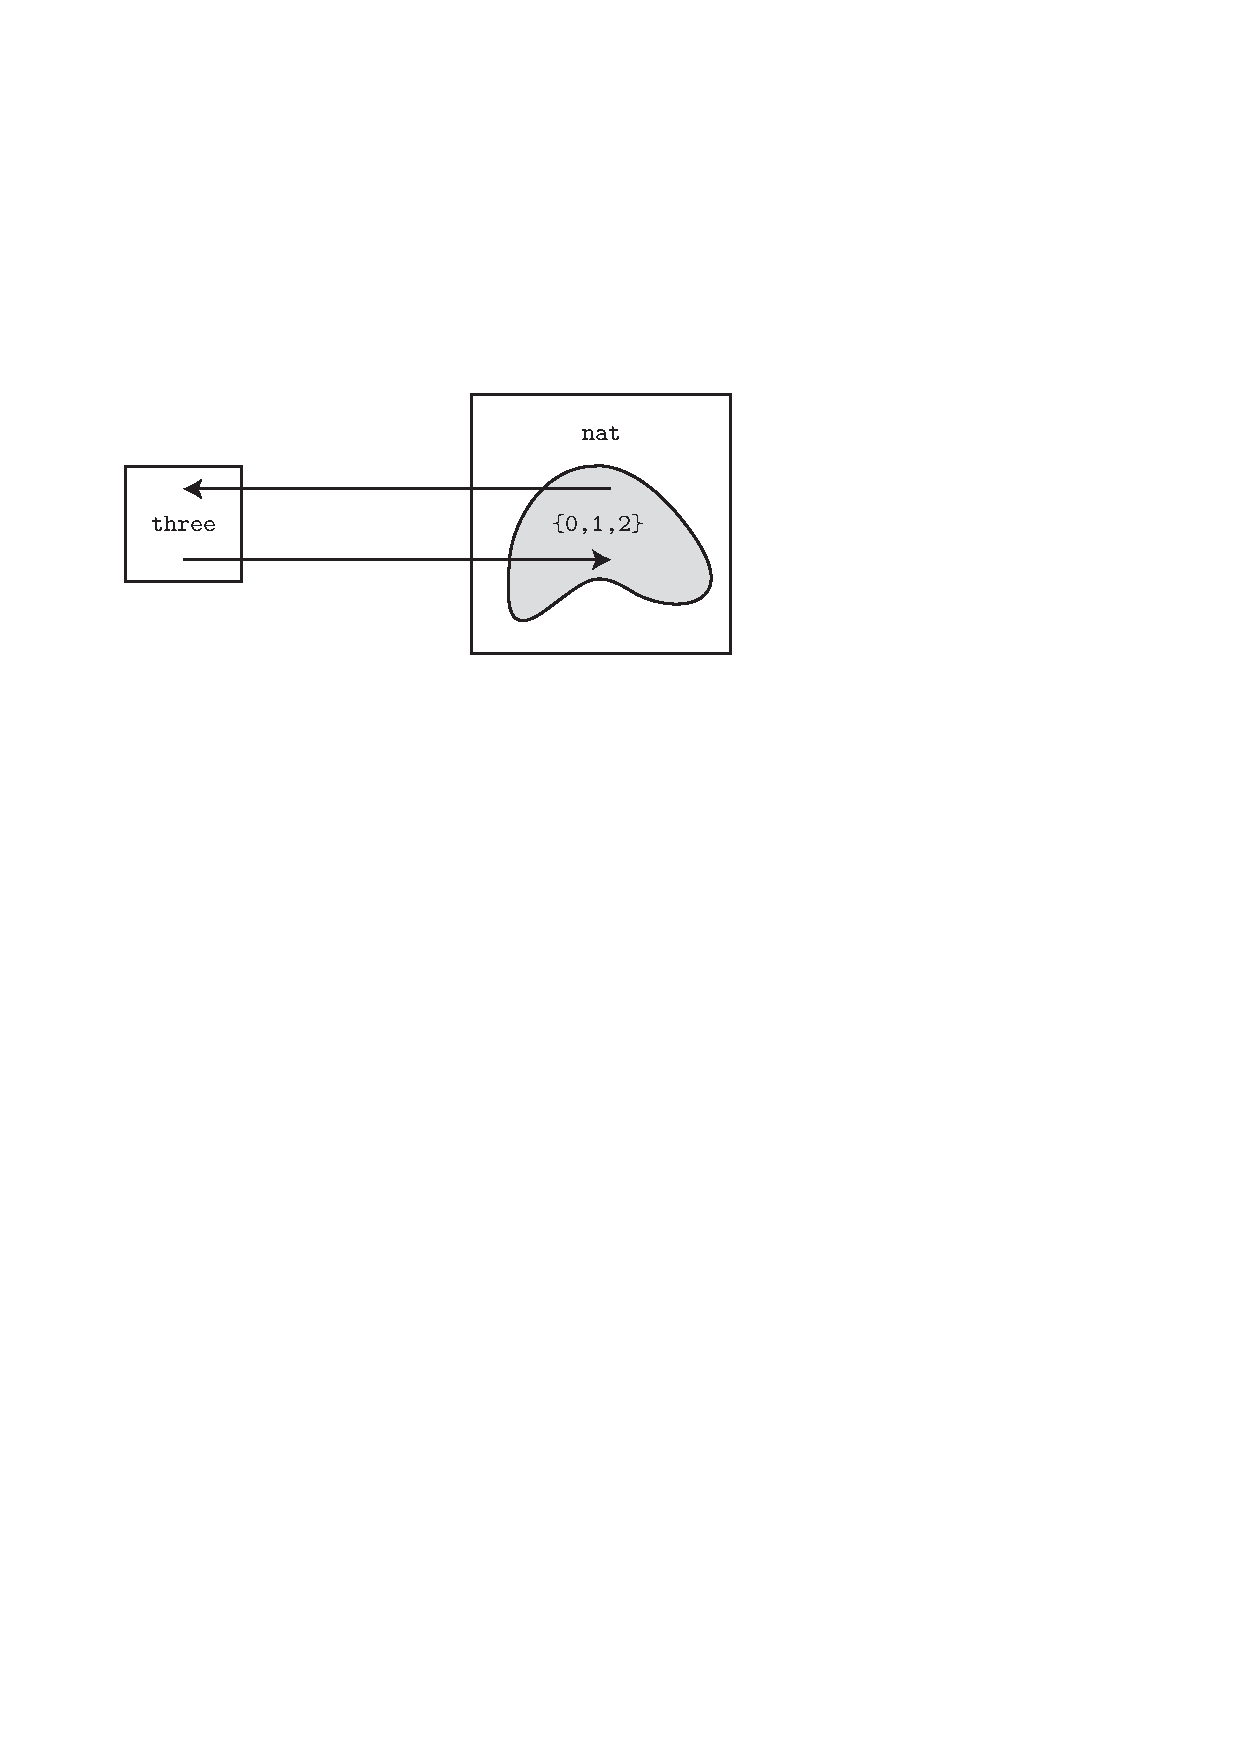
\includegraphics[scale=.8]{typedef}
\end{center}
Finally, \isacommand{typedef} asserts that \isa{Rep{\isacharunderscore}three} is
surjective on the subset \isa{three} and \isa{Abs{\isacharunderscore}three} and \isa{Rep{\isacharunderscore}three} are inverses of each other:
\begin{center}
\begin{tabular}{@ {}r@ {\qquad\qquad}l@ {}}
\isa{Rep{\isacharunderscore}three\ x\ {\isasymin}\ three} & (\isa{Rep{\isacharunderscore}three}) \\
\isa{Abs{\isacharunderscore}three\ {\isacharparenleft}Rep{\isacharunderscore}three\ x{\isacharparenright}\ {\isacharequal}\ x} & (\isa{Rep{\isacharunderscore}three{\isacharunderscore}inverse}) \\
\isa{y\ {\isasymin}\ three\ {\isasymLongrightarrow}\ Rep{\isacharunderscore}three\ {\isacharparenleft}Abs{\isacharunderscore}three\ y{\isacharparenright}\ {\isacharequal}\ y} & (\isa{Abs{\isacharunderscore}three{\isacharunderscore}inverse})
\end{tabular}
\end{center}
%
From this example it should be clear what \isacommand{typedef} does
in general given a name (here \isa{three}) and a set
(here \isa{{\isacharbraceleft}{\isadigit{0}}{\isacharcomma}\ {\isadigit{1}}{\isacharcomma}\ {\isadigit{2}}{\isacharbraceright}}).

Our next step is to define the basic functions expected on the new type.
Although this depends on the type at hand, the following strategy works well:
\begin{itemize}
\item define a small kernel of basic functions that can express all other
functions you anticipate.
\item define the kernel in terms of corresponding functions on the
representing type using \isa{Abs} and \isa{Rep} to convert between the
two levels.
\end{itemize}
In our example it suffices to give the three elements of type \isa{three}
names:%
\end{isamarkuptext}%
\isamarkuptrue%
\isacommand{constdefs}\isanewline
\ \ A{\isacharcolon}{\isacharcolon}\ three\isanewline
\ {\isachardoublequote}A\ {\isasymequiv}\ Abs{\isacharunderscore}three\ {\isadigit{0}}{\isachardoublequote}\isanewline
\ \ B{\isacharcolon}{\isacharcolon}\ three\isanewline
\ {\isachardoublequote}B\ {\isasymequiv}\ Abs{\isacharunderscore}three\ {\isadigit{1}}{\isachardoublequote}\isanewline
\ \ C\ {\isacharcolon}{\isacharcolon}\ three\isanewline
\ {\isachardoublequote}C\ {\isasymequiv}\ Abs{\isacharunderscore}three\ {\isadigit{2}}{\isachardoublequote}\isamarkupfalse%
%
\begin{isamarkuptext}%
So far, everything was easy. But it is clear that reasoning about \isa{three} will be hell if we have to go back to \isa{nat} every time. Thus our
aim must be to raise our level of abstraction by deriving enough theorems
about type \isa{three} to characterize it completely. And those theorems
should be phrased in terms of \isa{A}, \isa{B} and \isa{C}, not \isa{Abs{\isacharunderscore}three} and \isa{Rep{\isacharunderscore}three}. Because of the simplicity of the example,
we merely need to prove that \isa{A}, \isa{B} and \isa{C} are distinct
and that they exhaust the type.

In processing our \isacommand{typedef} declaration, 
Isabelle proves several helpful lemmas. The first two
express injectivity of \isa{Rep{\isacharunderscore}three} and \isa{Abs{\isacharunderscore}three}:
\begin{center}
\begin{tabular}{@ {}r@ {\qquad}l@ {}}
\isa{{\isacharparenleft}Rep{\isacharunderscore}three\ x\ {\isacharequal}\ Rep{\isacharunderscore}three\ y{\isacharparenright}\ {\isacharequal}\ {\isacharparenleft}x\ {\isacharequal}\ y{\isacharparenright}} & (\isa{Rep{\isacharunderscore}three{\isacharunderscore}inject}) \\
\begin{tabular}{@ {}l@ {}}
\isa{{\isasymlbrakk}x\ {\isasymin}\ three{\isacharsemicolon}\ y\ {\isasymin}\ three\ {\isasymrbrakk}} \\
\isa{{\isasymLongrightarrow}\ {\isacharparenleft}Abs{\isacharunderscore}three\ x\ {\isacharequal}\ Abs{\isacharunderscore}three\ y{\isacharparenright}\ {\isacharequal}\ {\isacharparenleft}x\ {\isacharequal}\ y{\isacharparenright}}
\end{tabular} & (\isa{Abs{\isacharunderscore}three{\isacharunderscore}inject}) \\
\end{tabular}
\end{center}
The following ones allow to replace some \isa{x{\isacharcolon}{\isacharcolon}three} by
\isa{Abs{\isacharunderscore}three{\isacharparenleft}y{\isacharcolon}{\isacharcolon}nat{\isacharparenright}}, and conversely \isa{y} by \isa{Rep{\isacharunderscore}three\ x}:
\begin{center}
\begin{tabular}{@ {}r@ {\qquad}l@ {}}
\isa{{\isasymlbrakk}y\ {\isasymin}\ three{\isacharsemicolon}\ {\isasymAnd}x{\isachardot}\ y\ {\isacharequal}\ Rep{\isacharunderscore}three\ x\ {\isasymLongrightarrow}\ P{\isasymrbrakk}\ {\isasymLongrightarrow}\ P} & (\isa{Rep{\isacharunderscore}three{\isacharunderscore}cases}) \\
\isa{{\isacharparenleft}{\isasymAnd}y{\isachardot}\ {\isasymlbrakk}x\ {\isacharequal}\ Abs{\isacharunderscore}three\ y{\isacharsemicolon}\ y\ {\isasymin}\ three{\isasymrbrakk}\ {\isasymLongrightarrow}\ P{\isacharparenright}\ {\isasymLongrightarrow}\ P} & (\isa{Abs{\isacharunderscore}three{\isacharunderscore}cases}) \\
\isa{{\isasymlbrakk}y\ {\isasymin}\ three{\isacharsemicolon}\ {\isasymAnd}x{\isachardot}\ P\ {\isacharparenleft}Rep{\isacharunderscore}three\ x{\isacharparenright}{\isasymrbrakk}\ {\isasymLongrightarrow}\ P\ y} & (\isa{Rep{\isacharunderscore}three{\isacharunderscore}induct}) \\
\isa{{\isacharparenleft}{\isasymAnd}y{\isachardot}\ y\ {\isasymin}\ three\ {\isasymLongrightarrow}\ P\ {\isacharparenleft}Abs{\isacharunderscore}three\ y{\isacharparenright}{\isacharparenright}\ {\isasymLongrightarrow}\ P\ x} & (\isa{Abs{\isacharunderscore}three{\isacharunderscore}induct}) \\
\end{tabular}
\end{center}
These theorems are proved for any type definition, with \isa{three}
replaced by the name of the type in question.

Distinctness of \isa{A}, \isa{B} and \isa{C} follows immediately
if we expand their definitions and rewrite with the injectivity
of \isa{Abs{\isacharunderscore}three}:%
\end{isamarkuptext}%
\isamarkuptrue%
\isacommand{lemma}\ {\isachardoublequote}A\ {\isasymnoteq}\ B\ {\isasymand}\ B\ {\isasymnoteq}\ A\ {\isasymand}\ A\ {\isasymnoteq}\ C\ {\isasymand}\ C\ {\isasymnoteq}\ A\ {\isasymand}\ B\ {\isasymnoteq}\ C\ {\isasymand}\ C\ {\isasymnoteq}\ B{\isachardoublequote}\isanewline
\isamarkupfalse%
\isacommand{by}{\isacharparenleft}simp\ add{\isacharcolon}\ Abs{\isacharunderscore}three{\isacharunderscore}inject\ A{\isacharunderscore}def\ B{\isacharunderscore}def\ C{\isacharunderscore}def\ three{\isacharunderscore}def{\isacharparenright}\isamarkupfalse%
%
\begin{isamarkuptext}%
\noindent
Of course we rely on the simplifier to solve goals like \isa{{\isadigit{0}}\ {\isasymnoteq}\ {\isadigit{1}}}.

The fact that \isa{A}, \isa{B} and \isa{C} exhaust type \isa{three} is
best phrased as a case distinction theorem: if you want to prove \isa{P\ x}
(where \isa{x} is of type \isa{three}) it suffices to prove \isa{P\ A},
\isa{P\ B} and \isa{P\ C}:%
\end{isamarkuptext}%
\isamarkuptrue%
\isacommand{lemma}\ three{\isacharunderscore}cases{\isacharcolon}\ {\isachardoublequote}{\isasymlbrakk}\ P\ A{\isacharsemicolon}\ P\ B{\isacharsemicolon}\ P\ C\ {\isasymrbrakk}\ {\isasymLongrightarrow}\ P\ x{\isachardoublequote}\isamarkupfalse%
%
\begin{isamarkuptxt}%
\noindent Again this follows easily from a pre-proved general theorem:%
\end{isamarkuptxt}%
\isamarkuptrue%
\isacommand{apply}{\isacharparenleft}induct{\isacharunderscore}tac\ x\ rule{\isacharcolon}\ Abs{\isacharunderscore}three{\isacharunderscore}induct{\isacharparenright}\isamarkupfalse%
%
\begin{isamarkuptxt}%
\begin{isabelle}%
\ {\isadigit{1}}{\isachardot}\ {\isasymAnd}y{\isachardot}\ {\isasymlbrakk}P\ A{\isacharsemicolon}\ P\ B{\isacharsemicolon}\ P\ C{\isacharsemicolon}\ y\ {\isasymin}\ three{\isasymrbrakk}\ {\isasymLongrightarrow}\ P\ {\isacharparenleft}Abs{\isacharunderscore}three\ y{\isacharparenright}%
\end{isabelle}
Simplification with \isa{three{\isacharunderscore}def} leads to the disjunction \isa{y\ {\isacharequal}\ {\isadigit{0}}\ {\isasymor}\ y\ {\isacharequal}\ {\isadigit{1}}\ {\isasymor}\ y\ {\isacharequal}\ {\isadigit{2}}} which \isa{auto} separates into three
subgoals, each of which is easily solved by simplification:%
\end{isamarkuptxt}%
\isamarkuptrue%
\isacommand{apply}{\isacharparenleft}auto\ simp\ add{\isacharcolon}\ three{\isacharunderscore}def\ A{\isacharunderscore}def\ B{\isacharunderscore}def\ C{\isacharunderscore}def{\isacharparenright}\isanewline
\isamarkupfalse%
\isacommand{done}\isamarkupfalse%
%
\begin{isamarkuptext}%
\noindent
This concludes the derivation of the characteristic theorems for
type \isa{three}.

The attentive reader has realized long ago that the
above lengthy definition can be collapsed into one line:%
\end{isamarkuptext}%
\isamarkuptrue%
\isacommand{datatype}\ better{\isacharunderscore}three\ {\isacharequal}\ A\ {\isacharbar}\ B\ {\isacharbar}\ C\isamarkupfalse%
%
\begin{isamarkuptext}%
\noindent
In fact, the \isacommand{datatype} command performs internally more or less
the same derivations as we did, which gives you some idea what life would be
like without \isacommand{datatype}.

Although \isa{three} could be defined in one line, we have chosen this
example to demonstrate \isacommand{typedef} because its simplicity makes the
key concepts particularly easy to grasp. If you would like to see a
non-trivial example that cannot be defined more directly, we recommend the
definition of \emph{finite multisets} in the Library~\cite{HOL-Library}.

Let us conclude by summarizing the above procedure for defining a new type.
Given some abstract axiomatic description $P$ of a type $ty$ in terms of a
set of functions $F$, this involves three steps:
\begin{enumerate}
\item Find an appropriate type $\tau$ and subset $A$ which has the desired
  properties $P$, and make a type definition based on this representation.
\item Define the required functions $F$ on $ty$ by lifting
analogous functions on the representation via $Abs_ty$ and $Rep_ty$.
\item Prove that $P$ holds for $ty$ by lifting $P$ from the representation.
\end{enumerate}
You can now forget about the representation and work solely in terms of the
abstract functions $F$ and properties $P$.%
\index{typedecl@\isacommand {typedef} (command)|)}%
\index{types!defining|)}%
\end{isamarkuptext}%
\isamarkuptrue%
\isamarkupfalse%
\end{isabellebody}%
%%% Local Variables:
%%% mode: latex
%%% TeX-master: "root"
%%% End:
    %%%Section "Introducing New Types"
